\documentclass[english,floatsintext,man]{apa6}

\usepackage{amssymb,amsmath}
\usepackage{ifxetex,ifluatex}
\usepackage{fixltx2e} % provides \textsubscript
\ifnum 0\ifxetex 1\fi\ifluatex 1\fi=0 % if pdftex
  \usepackage[T1]{fontenc}
  \usepackage[utf8]{inputenc}
\else % if luatex or xelatex
  \ifxetex
    \usepackage{mathspec}
    \usepackage{xltxtra,xunicode}
  \else
    \usepackage{fontspec}
  \fi
  \defaultfontfeatures{Mapping=tex-text,Scale=MatchLowercase}
  \newcommand{\euro}{€}
\fi
% use upquote if available, for straight quotes in verbatim environments
\IfFileExists{upquote.sty}{\usepackage{upquote}}{}
% use microtype if available
\IfFileExists{microtype.sty}{\usepackage{microtype}}{}

% Table formatting
\usepackage{longtable, booktabs}
\usepackage{lscape}
% \usepackage[counterclockwise]{rotating}   % Landscape page setup for large tables
\usepackage{multirow}		% Table styling
\usepackage{tabularx}		% Control Column width
\usepackage[flushleft]{threeparttable}	% Allows for three part tables with a specified notes section
\usepackage{threeparttablex}            % Lets threeparttable work with longtable

% Create new environments so endfloat can handle them
% \newenvironment{ltable}
%   {\begin{landscape}\begin{center}\begin{threeparttable}}
%   {\end{threeparttable}\end{center}\end{landscape}}

\newenvironment{lltable}
  {\begin{landscape}\begin{center}\begin{ThreePartTable}}
  {\end{ThreePartTable}\end{center}\end{landscape}}




% The following enables adjusting longtable caption width to table width
% Solution found at http://golatex.de/longtable-mit-caption-so-breit-wie-die-tabelle-t15767.html
\makeatletter
\newcommand\LastLTentrywidth{1em}
\newlength\longtablewidth
\setlength{\longtablewidth}{1in}
\newcommand\getlongtablewidth{%
 \begingroup
  \ifcsname LT@\roman{LT@tables}\endcsname
  \global\longtablewidth=0pt
  \renewcommand\LT@entry[2]{\global\advance\longtablewidth by ##2\relax\gdef\LastLTentrywidth{##2}}%
  \@nameuse{LT@\roman{LT@tables}}%
  \fi
\endgroup}


\ifxetex
  \usepackage[setpagesize=false, % page size defined by xetex
              unicode=false, % unicode breaks when used with xetex
              xetex]{hyperref}
\else
  \usepackage[unicode=true]{hyperref}
\fi
\hypersetup{breaklinks=true,
            pdfauthor={},
            pdftitle={The growth of children's semantic and phonological networks: insight from 10 languages},
            colorlinks=true,
            citecolor=blue,
            urlcolor=blue,
            linkcolor=black,
            pdfborder={0 0 0}}
\urlstyle{same}  % don't use monospace font for urls

\setlength{\parindent}{0pt}
%\setlength{\parskip}{0pt plus 0pt minus 0pt}

\setlength{\emergencystretch}{3em}  % prevent overfull lines

\ifxetex
  \usepackage{polyglossia}
  \setmainlanguage{}
\else
  \usepackage[english]{babel}
\fi

% Manuscript styling
\captionsetup{font=singlespacing,justification=justified}
\usepackage{csquotes}
\usepackage{upgreek}

 % Line numbering
  \usepackage{lineno}
  \linenumbers


\usepackage{tikz} % Variable definition to generate author note

% fix for \tightlist problem in pandoc 1.14
\providecommand{\tightlist}{%
  \setlength{\itemsep}{0pt}\setlength{\parskip}{0pt}}

% Essential manuscript parts
  \title{The growth of children's semantic and phonological networks: insight
from 10 languages}

  \shorttitle{Lexical Development as Network Growth}


  \author{Abdellah Fourtassi\textsuperscript{1}, Yuan Bian\textsuperscript{2}, \& Michael C. Frank\textsuperscript{1}}

  % \def\affdep{{"", "", ""}}%
  % \def\affcity{{"", "", ""}}%

  \affiliation{
    \vspace{0.5cm}
          \textsuperscript{1} Department of Psychology, Stanford University\\
          \textsuperscript{2} Department of Brain and Cognitive Sciences, Massachusetts Institute of
Technology  }

  \authornote{
    Abdellah Fourtassi
    
    Department of Psychology
    
    Stanford University
    
    50 Serra Mall
    
    Jordan Hall, Building 420
    
    Stanford, CA 94301
    
    Correspondence concerning this article should be addressed to Abdellah
    Fourtassi, Postal address. E-mail:
    \href{mailto:afourtas@stanford.edu}{\nolinkurl{afourtas@stanford.edu}}
  }


  \abstract{Children tend to produce words earlier when they are connected to a
variety of other words along the phonological and semantic dimensions.
Though these semantic and phonological connectivity effects have been
extensively documented, little is known about their underlying
developmental mechanism. One possibility is that learning is driven by
lexical network growth where highly connected words in the child's early
lexicon enable learning of similar words. Another possibility is that
learning is driven by highly connected words in the external learning
environment, instead of highly connected words in the early internal
lexicon. The present study tests both scenarios systematically in both
the phonological and semantic domains across 10 languages. We show that
phonological and semantic connectivity in the learning environment
drives growth in both production- and comprehension-based vocabularies,
even controlling for word frequency and length. This pattern of findings
suggests a word learning process where children harness their
statistical learning abilities to detect and learn highly connected
words in the learning environment.}
  \keywords{Word learning; semantic network; phonological network; network growth;
cross-linguistic analysis. \\

    
  }




  \usepackage[sortcites=false,sorting=none]{biblatex}

\usepackage{amsthm}
\newtheorem{theorem}{Theorem}
\newtheorem{lemma}{Lemma}
\theoremstyle{definition}
\newtheorem{definition}{Definition}
\newtheorem{corollary}{Corollary}
\newtheorem{proposition}{Proposition}
\theoremstyle{definition}
\newtheorem{example}{Example}
\theoremstyle{definition}
\newtheorem{exercise}{Exercise}
\theoremstyle{remark}
\newtheorem*{remark}{Remark}
\newtheorem*{solution}{Solution}
\begin{document}

\maketitle

\setcounter{secnumdepth}{0}



\section{Introduction}\label{introduction}

What factors shape vocabulary learning over the course of early
childhood? To investigate this question, scientists have adopted
multiple research strategies, from conducting controlled laboratory
experiments (e.g. Markman, 1990) to analyzing dense corpora capturing
language learning in context (e.g., B. C. Roy, Frank, DeCamp, Miller, \&
Roy, 2015). One prominent strategy consists in documenting the timeline
of words' acquisition and studying the properties that make words easy
or hard to learn (e.g., J. C. Goodman, Dale, \& Li, 2008; Huttenlocher,
Haight, Bryk, Seltzer, \& Lyons, 1991). For example, J. C. Goodman et
al. (2008) found that, within a lexical category (e.g., nouns), higher
parental frequency is associated with earlier learning. Researchers have
studied the role of several other factors such as word length and the
mean length of utterances in which the word occurs (e.g., Braginsky,
Yurovsky, Marchman, \& Frank, 2019; Swingley \& Humphrey, 2018).

Besides word-level properties, the structure of the lexicon (that is,
how words relate to one another) is also linked to the Age of
Acquisition (AoA) of words. The lexical structure can be characterized
in terms of a network where each node represents a word in the
vocabulary, and each link between two nodes represents a relationship
between the corresponding pair of words (e.g., Collins \& Loftus, 1975;
Luce \& Pisoni, 1998). Previous studies have investigated early
vocabulary structure by constructing networks using a variety of
word-word relations including shared semantic features (McRae, Cree,
Seidenberg, \& McNorgan, 2005), target-cue relationships in free
association norms (Nelson, McEvoy, \& Schreiber, 1998), co-occurrence in
child-directed speech (MacWhinney, 2014), and phonological relatedness
(Vitevitch, 2008). These studies have generally found that children tend
to produce words that have higher neighborhood density (i.e., high
connectivity in the network) earlier, both at the phonological and the
semantic level (Carlson, Sonderegger, \& Bane, 2014; Hills, Maouene,
Riordan, \& Smith, 2010; Hills, Maouene, Maouene, Sheya, \& Smith, 2009;
Stella, Beckage, \& Brede, 2017; Storkel, 2009).

While most studies have focused on the static properties of the lexical
network, a few have investigated the underlying developmental process.
In particular, Steyvers and Tenenbaum (2005) suggested that the observed
effects of connectivity are the consequence of how the lexical network
gets constructed in the child's mind. According to this explanation,
known as Preferential Attachment, highly connected words in the child's
lexicon tend to \enquote{attract} more words over time, in a
rich-get-richer scenario (Barabasi \& Albert, 1999). In other words,
what predicts learning is the \emph{internal} connectivity in the
child's early lexicon. In contrast, Hills et al. (2009) suggested that
what biases the learning is not the connectivity in the child's internal
lexicon but, rather, \emph{external} connectivity in the learning
environment. They called this alternative explanation Preferential
Acquisition. For clarity of reading, we will call preferential
attachment the Internally-driven mechanism (INT), and preferential
acquisition the Externally-driven mechanism (EXT).
Figure~\ref{fig:growth} shows an illustration of both growth scenarios
with the same simplified network.

These two proposals represent two divergent ideas about the role of
lexical networks in acquisition. On the INT proposal, learning is driven
by known words with high connectivity to other known words (Figure 1,
left). Thus, the network structure is a causal factor in word learning,
that is, children rely on the organization of their past knowledge to
determine future learning (Altvater-Mackensen \& Mani, 2013; Borovsky,
Ellis, Evans, \& Elman, 2016; Chi \& Koeske, 1983; Storkel, 2009). In
contrast, on the EXT approach, learning is driven by the connectivity of
words that are not known yet (Figure 1, right). Thus, the relevant
network structure is not internally represented by children, and the
observed connectivity effect might be an epiphenomenon of some
properties of the linguistic input. For example, highly connected
concrete nouns in the input could be more easily learned because of
their contextual diversity, allowing for easier meaning disambiguation
(McMurray, Horst, \& Samuelson, 2012; Smith \& Yu, 2008; Yurovsky \&
Frank, 2015). Another reason could be that these words are emphasized by
the caregivers in their child-directed speech (Clark, 2007; Hoff \&
Naigles, 2002; Huttenlocher et al., 1991).

\begin{figure}

{\centering 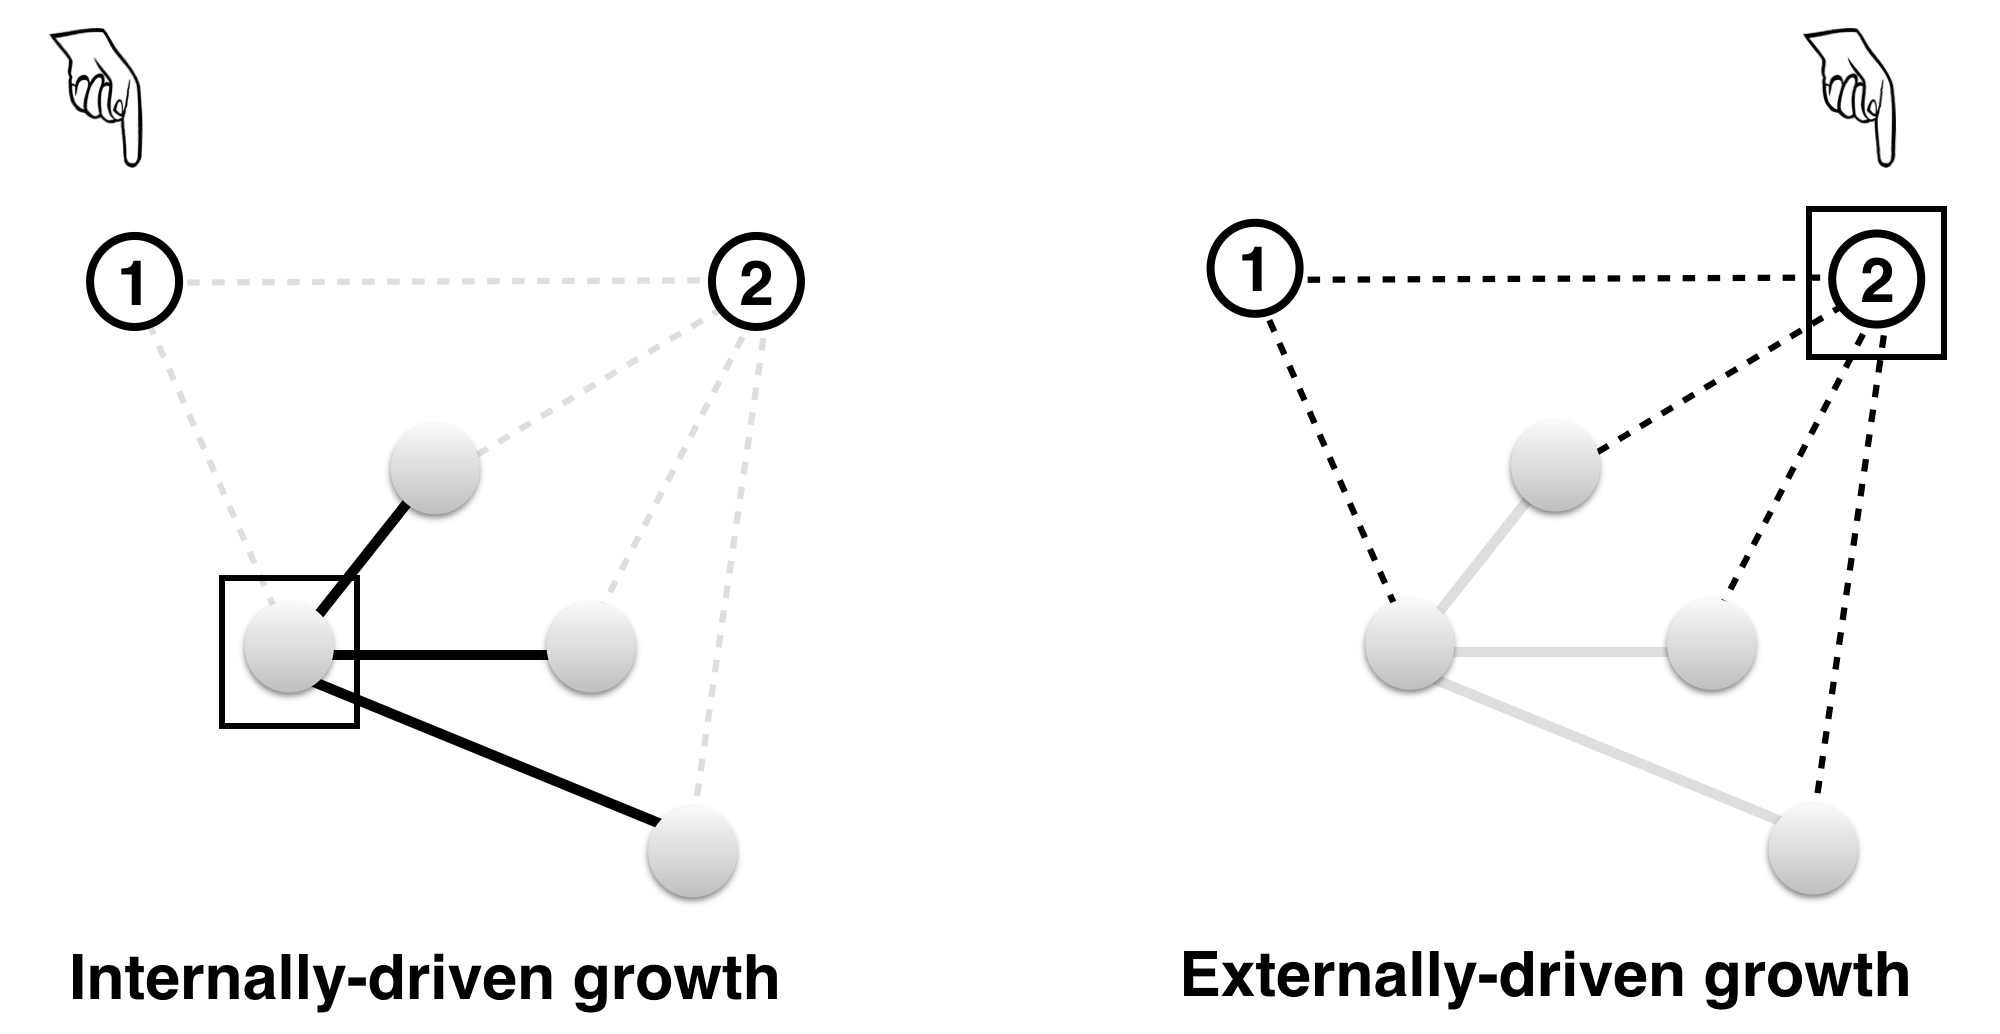
\includegraphics[width=300px]{figs/growth3} 

}

\caption{Illustration of the two growth scenarios. Filled grey circles represent known words (Internal) at a certain point in time. The empty, numbered circles represent words that have not yet been learned (External) and which are candidates to enter the lexicon next. The identity of the word that is going to be learned depends on the growth scenario.  Here the squares indicate the node that drives growth in each scenario, and the hand pointer indicates which word is likely to be learned. For INT, the utility of a candidate external node is the average degree (i.e., number of links) of the internal nodes that it would attach to. In this simplified example, candidate node 1 would connect to an internal node with 3 connections; thus we have $u_{INT}(node_1)= 3$. As for candidate node 2, it would connect to internal nodes that have only one connection each, making an average of 1, i.e., $u_{INT}(node_2)= 1$. According to INT, node 1 is more likely to enter the lexicon. For EXT, the utility of a candidate node is its degree in the entire network. In our example, candidate node 1 has 2 connections in total, whereas candidate node 2 has 5 connections. So we have $u_{EXT}(node_1)= 2$ and $u_{EXT}(node_2)= 5$. Thus, according to EXT, node 2 is more likely to enter the lexicon next. This figure is based on an example from Hills et al. (2009).}\label{fig:growth}
\end{figure}

Hills et al. (2009) investigated the growth of lexico-semantic networks
in toddlers and found that growth did not proceed according to INT as
was originally hypothesized by Steyvers and Tenenbaum (2005), but rather
according to
EXT.\footnote{Besides INT and EXT, the authors tested a third mechanism (called the lure of associates) which resembles EXT in that it is driven by the connectivity of external nodes, except that this connectivity is computed with respect to words that are known. However, EXT is the externally-driven scenario that best predicted the data in this previous work.}
This is an important finding because it suggests that learning in the
early stages is mostly driven by properties of the external input,
regardless of how past knowledge is organized. However, this work
explored the INT/EXT growth in a special case: networks that were based
on 1) semantic associations, 2) production-based vocabularies, and 3)
data from English-learning children, only. The extent to which this
result depends on the domain (e.g., semantic vs.~phonological
connectivity), the vocabulary measure (production vs.~comprehension) and
culture/language is thus an open area for investigation (Hills \& Siew,
2018). In this work, we test the generality of prior findings along
these three dimensions.

First, we study the phonological network in addition to the semantic
network. These two networks represent different ways the mental lexicon
is structured (Beckage \& Colunga, 2016). In particular, words that are
neighbors in the semantic network (e.g., cat, dog) are not necessarily
neighbors in the phonological network and vice versa. Does the
phonological network also predict word learning? Previous work has found
an effect of words' connectivity in the phonological network on their
age of learning (Carlson et al., 2014; Stella et al., 2017; Storkel,
2009). In other words, words learned earlier in life tend to sound
similar to many other words than a word learned later in life. However,
this finding is \emph{a priori} compatible with both INT and EXT, and
previous studies did not explicitly compare these two mechanisms. Here,
we investigate whether phonological networks, like semantic networks,
grow through EXT, or if they rather grow via INT
(Figure~\ref{fig:growth}).

Second, we study vocabularies measured using both comprehension and
production. Previous studies have found differences between these
vocabularies in terms of their content and rate of acquisition (Bates,
Dale, \& Thal, 1995; Benedict, 1979; Fenson et al., 1994). These
differences may reflect the fact that comprehension and production do
not share the same constraints. For instance, whereas comprehension
depends on the ease with which words are stored and accessed, production
depends, additionally, on the ease with which words are articulated,
e.g., shorter words are produced earlier (Braginsky et al., 2019). By
investigating comprehension-based vocabularies, we assess the extent to
which the network growth mechanism captures general learning patterns
beyond the specific constraints of production.

Finally, we use developmental data in 10 languages. Lexical networks can
show more or less cross-linguistic variability along both the semantic
and phonological domains (Arbesman, Strogatz, \& Vitevitch, 2010; Lupyan
\& Lewis, 2017; Youn et al., 2016). Besides, cultures might differ in
the way caregivers talk to children (Cristia, Dupoux, Gurven, \&
Stieglitz, 2017; Kuhl et al., 1997), and this difference in the input
could influence the way in which the children's networks grow. Thus,
cross-linguistic comparison is crucial to test the extent to which
growth mechanisms are equally engaged across a wider variety of cultures
compared with the extent to which the growth mechanisms are specific to
patterns of learning that emerge due to the particulars of a given
language or culture (Bates \& MacWhinney, 1987; Slobin, 2014).

We adopted the following research strategy. We used parent reports on
the MacArthur-Bates Communicative Development Inventory and its
cross-linguistic adaptations (Fenson et al., 1994; Frank, Braginsky,
Yurovsky, \& Marchman, 2017). We studied the timeline of word learning
using the normative age of acquisition (i.e., the age at which at least
50\% of children know a given word). Our choice of studying the
normative learning trajectory rather than the individual trajectories
was motivated by the nature of the dataset used---which is primarily
based on cross-sectional studies. Children may vary in their individual
learning trajectories, but the aggregate data provide highly robust
measures of the average learning patterns (Fenson et al., 1994). The use
of such measures has lead to important insights on the mechanisms of
word learning (J. C. Goodman et al., 2008; Hills et al., 2010, 2009;
Stella et al., 2017; Storkel, 2009).

The paper is organized as follows. First, we describe the datasets we
used and explain how we constructed the networks. Second, we analyze
static properties of words' connectivity in these networks (correlation
with age of acquisition and shape of the distribution), and we explain
how these properties inform hypotheses about network growth. Next, we
fit the two hypothesized growth mechanisms to the data. We investigate
the extent to which the results obtained in Hills et al. (2009)
generalize to phonological networks and comprehension-based
vocabularies, and whether this generalization holds
cross-linguistically.

\section{Networks}\label{networks}

\subsection{Data}\label{data}

We used data from Wordbank (Frank et al., 2017), an open repository
aggregating cross-linguistic language developmental data of the
MacArthur-Bates Communicative Development Inventory (CDI), a parent
report vocabulary checklist. Parent report is a reliable and valid
measure of children's vocabulary that allows for the cost-effective
collection of datasets large enough to test network-based models of
acquisition (Fenson et al., 1994). When filling out a CDI form,
caregivers are either invited to indicate whether their child
\enquote{understands} (comprehension) or \enquote{understands and says}
(production) each of about 400-700 words. For younger children (e.g., 8
to 18 months in the English data), both comprehension and production are
queried, whereas for older children (16 to 36 months) only production is
queried. Due to these limitations, we use data from younger children to
test comprehension and data from older children to test production. In
addition, following previous studies (Hills et al., 2009; Storkel,
2009), we restricted our analysis to the category of nouns due to the
fact that nouns predominate the early expressive and receptive lexicons
(Bates et al., 1995). Their larger sample size (compared, for example,
to verbs or adjectives) is more suited to the network-based analysis of
development. Table \ref{tab:stats} gives an overview of the data we
used.

\subsection{Age of acquisition}\label{age-of-acquisition}

For each word in the CDI data, we compute the proportion of children who
understand or produce the word at each month. Then we fit a logistic
curve to these proportions and determined when the curve crosses 0.5,
i.e., the age at which at least 50\% of children know the word. We take
this point in time to be each word's age of acquisition (Braginsky et
al., 2019; J. C. Goodman et al., 2008).

\begin{table}

\caption{\label{tab:stats}Statistics for the dataset we used. The ages are in months.}
\centering
\begin{tabular}[t]{>{\bfseries}lrlrrlr}
\toprule
\multicolumn{1}{c}{} & \multicolumn{3}{c}{Comprehension} & \multicolumn{3}{c}{Production} \\
\cmidrule(l{2pt}r{2pt}){2-4} \cmidrule(l{2pt}r{2pt}){5-7}
Language & Nouns & Ages & N & Nouns & Ages & N\\
\midrule
Croatian & 209 & 8-16 & 250 & 312 & 16-30 & 377\\
Danish & 200 & 8-20 & 2,398 & 316 & 16-36 & 3,714\\
English & 209 & 8-18 & 2,435 & 312 & 16-30 & 5,520\\
French & 197 & 8-16 & 537 & 307 & 16-30 & 827\\
Italian & 209 & 7-24 & 648 & 312 & 18-36 & 752\\
Norwegian & 193 & 8-20 & 2,922 & 316 & 16-36 & 9,303\\
Russian & 207 & 8-18 & 768 & 314 & 18-36 & 1,037\\
Spanish & 208 & 8-18 & 788 & 312 & 16-30 & 1,146\\
Swedish & 205 & 8-16 & 467 & 339 & 16-28 & 900\\
Turkish & 180 & 8-16 & 1,115 & 297 & 16-36 & 2,422\\
\bottomrule
\end{tabular}
\end{table}

\subsection{Semantic networks}\label{semantic-networks}

We constructed semantic networks for English data following the
procedure outlined in Hills et al. (2009), as follows. We used as an
index of semantic relatedness the Florida Free Association Norms (Nelson
et al., 1998). This dataset was collected by giving adult participants a
word (the cue), and asking them to write the first word that comes to
mind (the target). For example, when given the word \enquote{ball,} they
might answer with the word \enquote{game.} A pair of nodes were
connected by a directed link from the cue to the target if there was a
cue-target relationship between these nodes in the association norms.
The connectivity of a given node was characterized by its
\emph{indegree}: the number of links for which the word was the
target.\footnote{This choice was based on prior work by Hills et al. (2009) stating that analyses with both outdegrees (sum of the links where the word is the cue in a cue-target pair) and total degree  (outdegree plus indegree) led to results weaker than those calculated with indegree.}
To model growth from month to month, we constructed a different network
at each month, based on the nouns that have been acquired by that month.

Since the free association norms are available only in English, we used
the hand-checked translation equivalents available in Wordbank, which
allowed us to use the English association norms across 10 languages.
Semantic associations are not necessarily shared across languages, but
we use this technique as a reasonable first approximation. In support of
this approximation, Youn et al. (2016) showed that semantic networks
across languages share substantial similarities. The fact that semantic
associations are assumed to be shared across languages does not mean
that the semantic networks will necessarily grow in a similar fashion.
For instance, the set of words acquired by children as well as the order
of word acquisition can vary from language to language leading to
possibily different learning strategies.

\subsection{Phonological networks}\label{phonological-networks}

To construct phonological networks we first mapped the orthographic
transcription of words to their International Phonetic Alphabet (IPA)
transcriptions in each language, using the open-source text-to-speech
software \textbf{\href{http://http://espeak.sourceforge.net/}{Espeak}}.
This software provides the correct IPA transcription if the word is
found in a spelling-to-phonemes dictionary, otherwise it uses
language-specific pronunciation rules to generate an approximate
phonetic transcription. We used the Levenshtein distance (also known as
edit distance) as a measure of phonological relatedness between two
nodes. The measure counts the minimum number of operations (insertions,
deletions, substitutions) required to change one string into another.

In previous studies, two nodes were linked if they had an edit distance
of 1 (Carlson et al., 2014; Stella et al., 2017; Storkel, 2009).
However, these studies reported a contribution of phonological
connectivity to noun learning when networks were built using a dense
adult vocabulary. Since the focus of the current study is on the
mechanism of growth, the networks are based on children's early
vocabulary. The latter, however, contains very few noun pairs with an
edit distance of 1. To better represent the similarity space in the
phonological domain, we increased the threshold from 1 to 2, that is,
two nodes were related if their edit distance was equal to 1 or
2.\footnote{In Appendix A, we show the main results for phonological networks based on an edit distance of 1. We also show the results for phonological networks where the edges between pairs of words were weighted by the inverse of the edit distance. We did not consider the case of a threshold larger than 2 since many short pairs appear phonologically unrelated when the edit distance is 3 or more (e.g., "cat"/"dog").}
The connectivity of a given node was characterized with its
\emph{degree}: the number of links it shares with other words.

\section{Analysis}\label{analysis}

\subsection{Static properties of the global
network}\label{static-properties-of-the-global-network}

We start by analyzing word connectivity in the global (static) network.
We constructed this network using nouns learned by the oldest age for
which we have CDI data (e.g., in English this corresponds, in
comprehension, to the network by 18 months, and in production, to the
network by 30 months). This global network is the end-state towards
which both INT and EXT converge by the last month of learning. Moreover,
following Hills et al. (2009), we used this end-state network as a proxy
for the external connectivity in the learning environment. Below we
analyze properties of these global networks that may a priori hint at an
INT- or EXT-like growth.

\begin{figure}[!h]
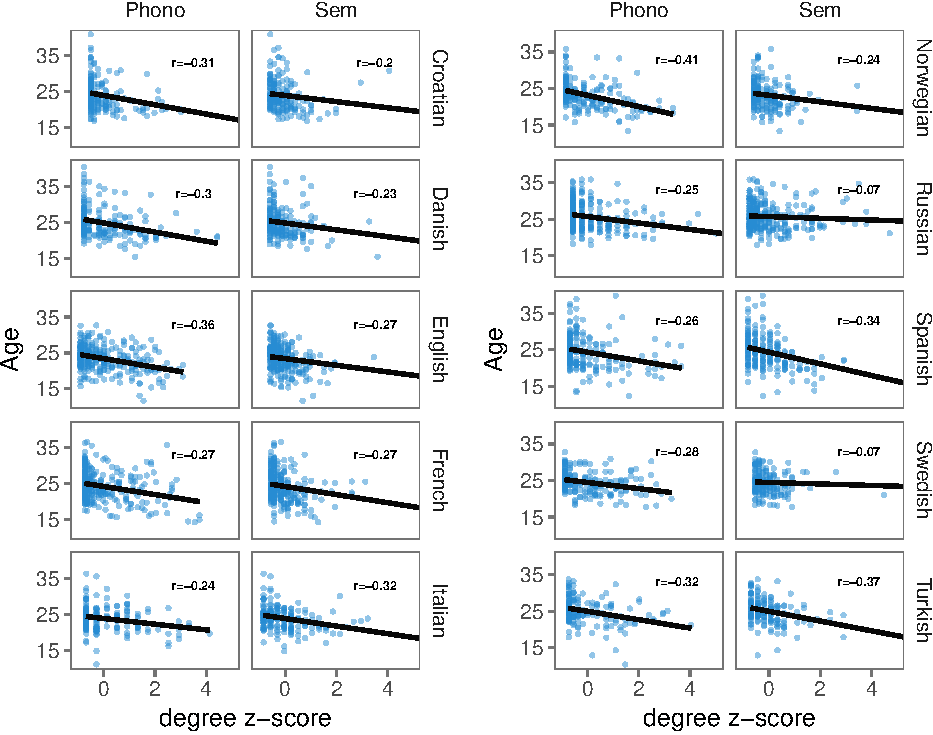
\includegraphics[width=\textwidth]{ms_files/figure-latex/corrProd-1} \caption{Production data (Age of acquisition) as predicted by the degree (i.e., connectivity) in this network. Results are shown in each language for phonological and semantic networks. Each point is a word, with lines indicating linear model fits, and numbers indicating the Pearson correlation coefficients.}\label{fig:corrProd}
\end{figure}

\begin{figure}[!h]
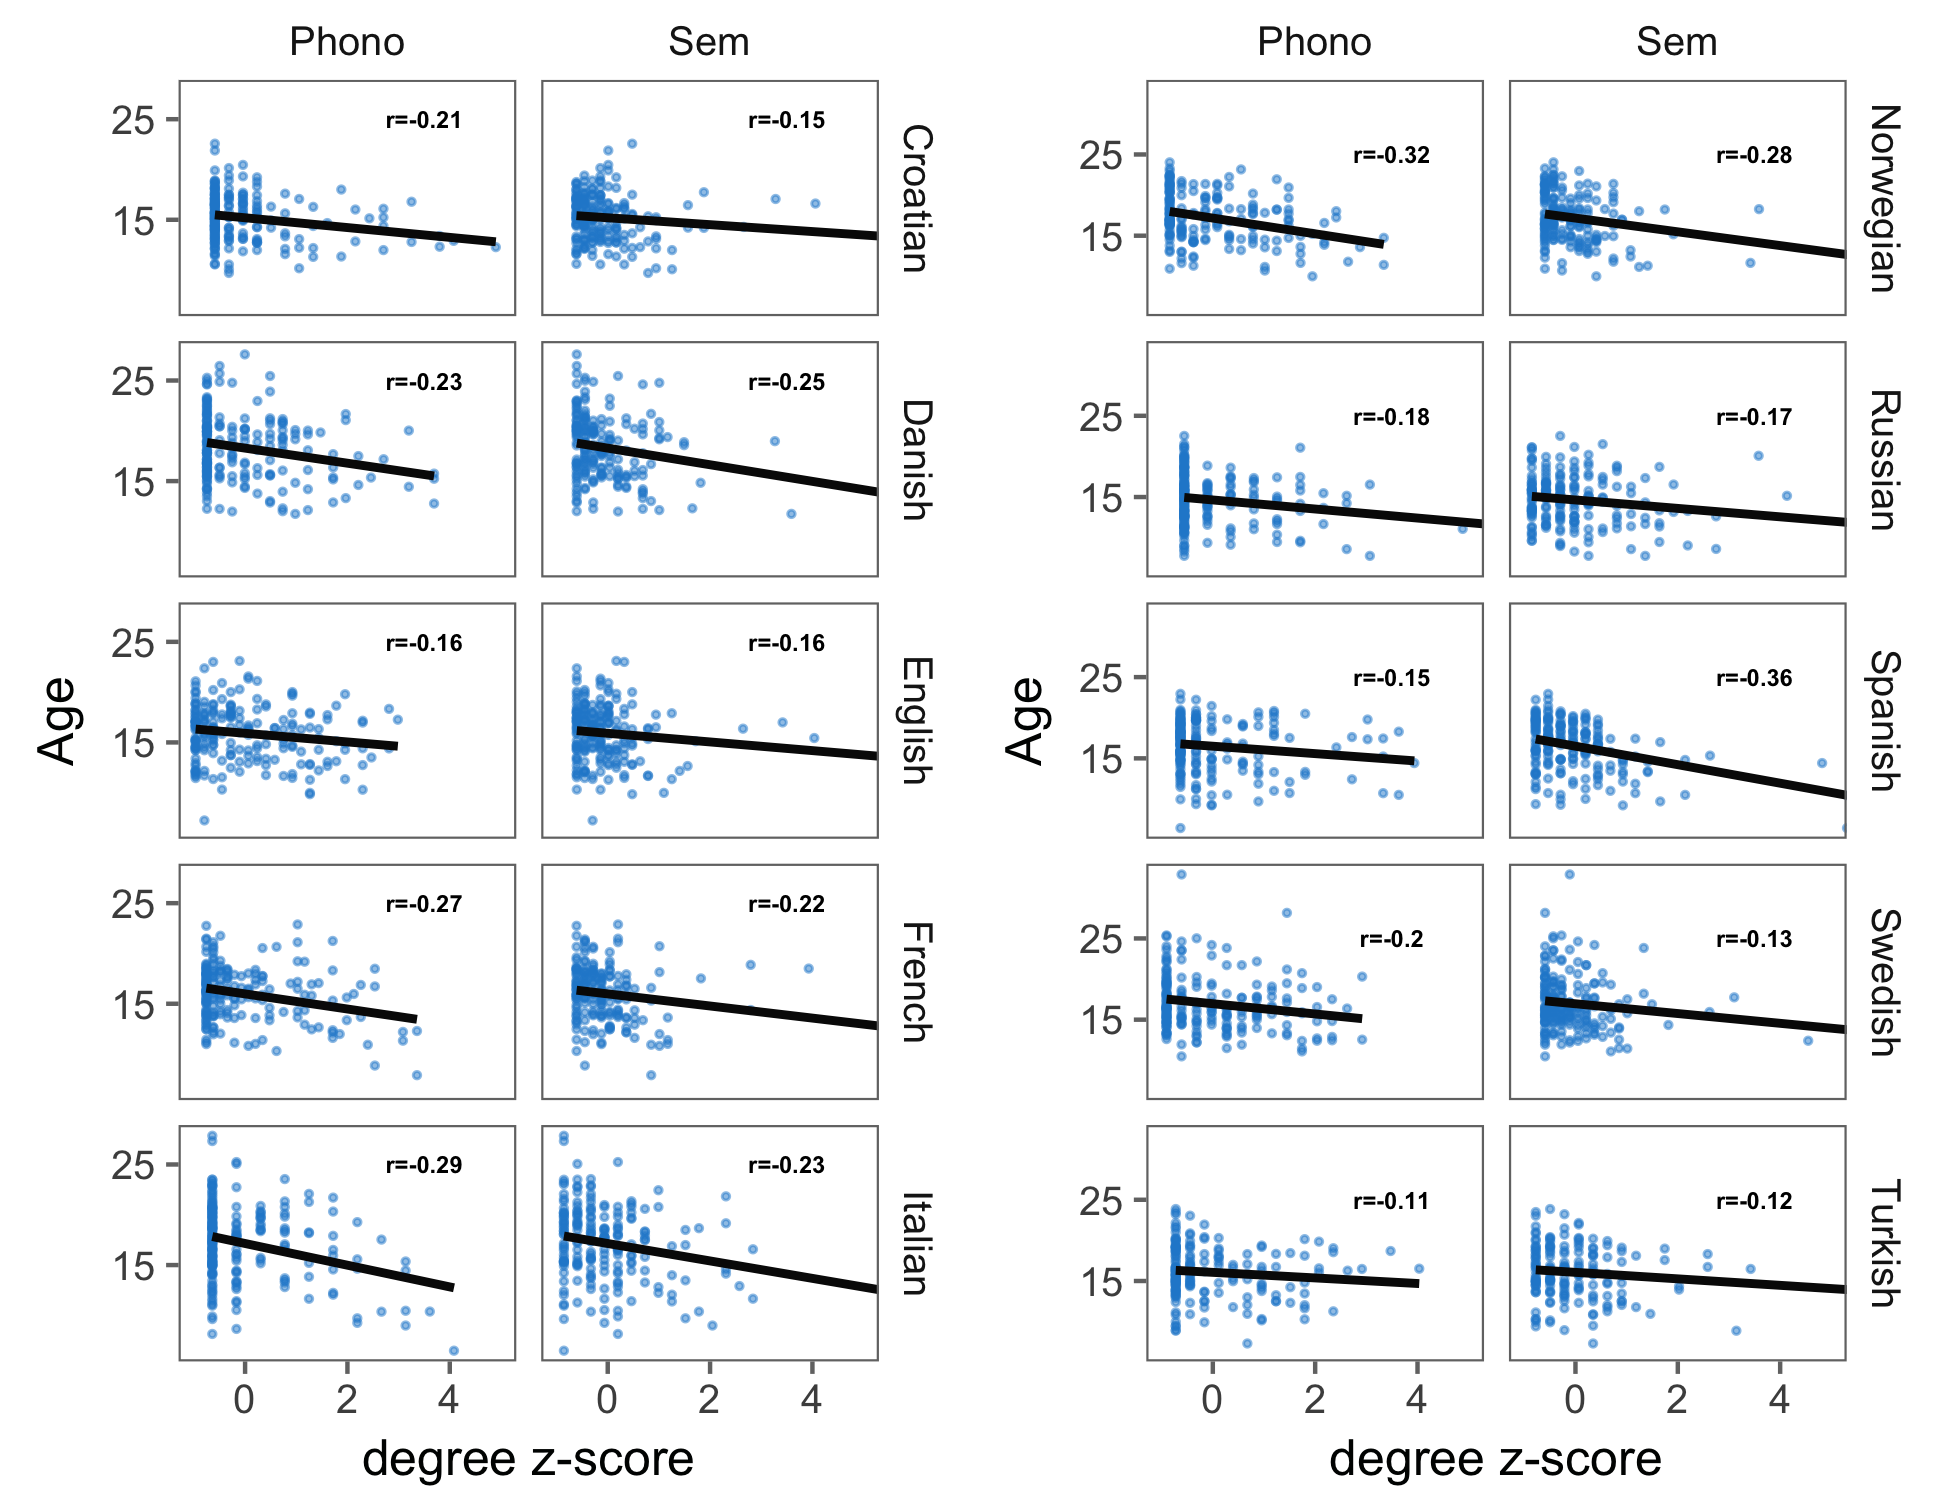
\includegraphics[width=\textwidth]{ms_files/figure-latex/corrComp-1} \caption{Comprehension data (Age of acquisition) as predicted by the degree (i.e., connectivity) in this network. Results are shown in each language for phonological and semantic networks. Each point is a word, with lines indicating linear model fits, and numbers indicating the Pearson correlation coefficients.}\label{fig:corrComp}
\end{figure}

\subsubsection{Connectivity predicts the age of
acquisition}\label{connectivity-predicts-the-age-of-acquisition}

Connectivity in the global network is directly related to EXT as it
represents the explicit criterion this growth scenario uses to determine
what words should be learned first (Figure \ref{fig:growth}). Therefore,
a direct consequence of an EXT-like growth scenario is a correlation
between connectivity in the global network and the age of acquisition.
This correlation is also necessary to INT, although the causality is
reversed: Higher connectivity in the global network is caused by earlier
learning, not the other way around. Some words end up being highly
connected in the global network precisely because they happen to be
acquired earlier and, therefore, have a higher chance of accumulating
more links over time. Thus, the correlation between connectivity in the
end-state network and AoA can result from both EXT and INT. If there is
no such correlation, neither growth scenario can be posited as a
possible learning mechanism.

Figures \ref{fig:corrProd} and \ref{fig:corrComp} show how the age of
acquisition in production and comprehension, respectively, correlates
with the degree (or indegree for the semantic networks). For ease of
visual comparison, the predictor (i.e., the degree) was centered and
scaled. The plots show, overall, a negative correlation between the
month of acquisition and the degree. In production data, the average
correlation across languages was -0.24 (\(SD=\) 0.10) for the semantic
networks and -0.30 (\(SD=\) 0.05) for the phonological networks. In
comprehension data, the average correlation was -0.21 (\(SD=\) 0.08) for
the semantic networks and -0.21 (\(SD=\) 0.07) for the phonological
networks. These results indicate that nouns with higher degrees are
generally learned earlier, thus replicating previous findings in English
(Hills et al., 2009; Storkel, 2009) and extending these findings to 10
different languages, generally, in both production- and
comprehension-based vocabularies.

\begin{figure}[!h]
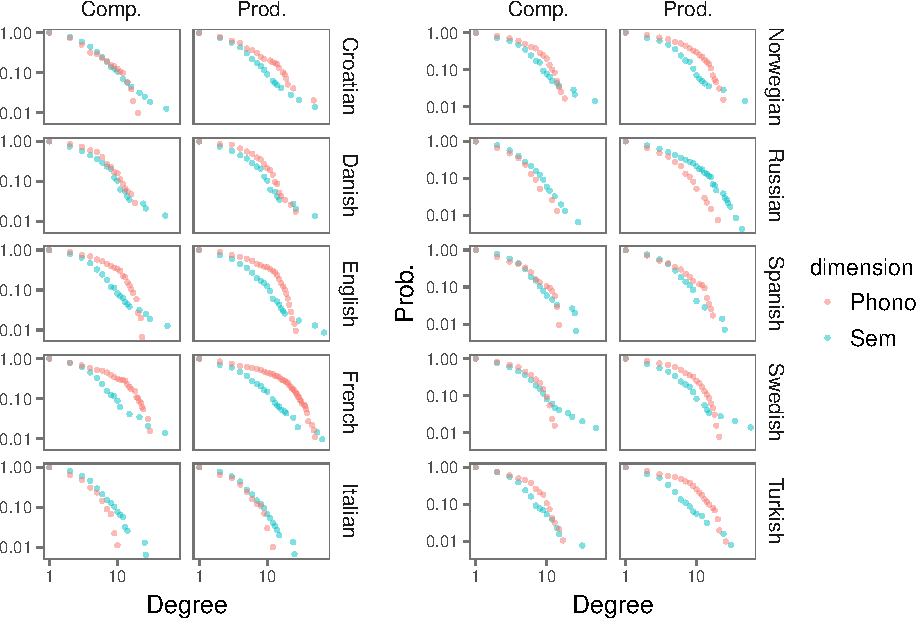
\includegraphics[width=\textwidth]{ms_files/figure-latex/degreeDist-1} \caption{Log-log plot of the cumulative degree distribution function for the global phonological and semantic networks across languages. The figure shows the results for both production and comprehension data. A perfect power-law distribution should appear as a straight line in this graph.}\label{fig:degreeDist}
\end{figure}

\subsubsection{Power-law degree
distribution}\label{power-law-degree-distribution}

We also analyzed the global network's degree distribution. The shape of
this distribution is particularly relevant to INT as this growth
scenario is known to generate networks with a power-law degree
distribution, i.e., a distribution of the form
\(p(k) \propto \frac{1}{k^{\alpha}}\) (Barabasi \& Albert, 1999). If the
end-state network displays this property, this fact would suggest, but
not prove, an INT-like generative process. If, however, the degree
distribution is very different from a power law, this would
significantly weaken the case for INT. The log-log plots are shown in
Figure \ref{fig:degreeDist}. We fit a power law to each empirical degree
distribution following the procedure outlined in Clauset, Shalizi, and
Newman (2009) and using a related R package (poweRlaw, Gillespie, 2015).

\begin{table}

\caption{\label{tab:powerLawProd}Results of fitting a power law model to the degree (i.e., connectivity) distribution in each model for production data. Numbers indicate the cut-off degree, the scaling parameter alpha, and the p-value which quantifies the plausibility of the power law hypothesis. If the p-value is close to 1, a power law cannot be rejected as a plausible fit for the data.}
\centering
\begin{tabular}[t]{>{\bfseries}lrrrrrr}
\toprule
\multicolumn{1}{c}{} & \multicolumn{3}{c}{Phono.} & \multicolumn{3}{c}{Sem.} \\
\cmidrule(l{2pt}r{2pt}){2-4} \cmidrule(l{2pt}r{2pt}){5-7}
Language & cut-off & alpha & p-value & cut-off & alpha & p-value\\
\midrule
Croatian & 4 & 2.18 & 0.123 & 4 & 2.55 & 0.881\\
Danish & 11 & 4.55 & 0.858 & 4 & 2.38 & 0.001\\
English & 20 & 9.14 & 0.511 & 5 & 2.66 & 0.132\\
French & 20 & 3.75 & 0.112 & 8 & 2.81 & 0.133\\
Italian & 9 & 9.45 & 0.780 & 4 & 2.93 & 0.608\\
Norwegian & 15 & 6.28 & 0.744 & 5 & 2.88 & 0.201\\
Russian & 8 & 4.20 & 0.541 & 24 & 5.61 & 0.723\\
Spanish & 13 & 8.75 & 0.736 & 4 & 2.98 & 0.460\\
Swedish & 11 & 4.68 & 0.103 & 4 & 2.49 & 0.171\\
Turkish & 8 & 3.26 & 0.375 & 4 & 2.87 & 0.925\\
\bottomrule
\end{tabular}
\end{table}

\begin{table}

\caption{\label{tab:powerLawComp}Results of fitting a power law model to the degree distribution in each model for comprehension data. Numbers indicate the cut-off degree, the scaling parameter alpha, and the p-value which quantifies the plausibility of the power law hypothesis. If the p-value is close to 1, a power law cannot be rejected as a plausible fit for the data.}
\centering
\begin{tabular}[t]{>{\bfseries}lrrrrrr}
\toprule
\multicolumn{1}{c}{} & \multicolumn{3}{c}{Phono.} & \multicolumn{3}{c}{Sem.} \\
\cmidrule(l{2pt}r{2pt}){2-4} \cmidrule(l{2pt}r{2pt}){5-7}
Language & cut-off & alpha & p-value & cut-off & alpha & p-value\\
\midrule
Croatian & 2 & 2.06 & 0.020 & 5 & 2.67 & 0.895\\
Danish & 5 & 2.98 & 0.136 & 4 & 2.39 & 0.005\\
English & 13 & 5.16 & 0.235 & 4 & 2.64 & 0.765\\
French & 18 & 5.58 & 0.336 & 4 & 2.63 & 0.330\\
Italian & 8 & 10.27 & 0.909 & 4 & 2.88 & 0.688\\
Norwegian & 13 & 7.65 & 0.440 & 5 & 2.87 & 0.433\\
Russian & 5 & 3.97 & 0.854 & 8 & 3.91 & 0.952\\
Spanish & 5 & 3.01 & 0.085 & 5 & 3.11 & 0.552\\
Swedish & 9 & 6.75 & 0.102 & 5 & 2.81 & 0.713\\
Turkish & 9 & 5.73 & 0.958 & 4 & 3.13 & 0.887\\
\bottomrule
\end{tabular}
\end{table}

In brief, the analysis consisted in two steps. First, we derived the
optimal cut-off, \(k_{min}\), above which the distribution is more
likely to follow a power
law,\footnote{In natural phenomena, it is often the case that the power law applies only for values above a certain minimum.}
and we estimate the corresponding scaling parameter \(\alpha\). Second,
we calculated the goodness-to-fit, which resulted in a \(p\)-value
quantifying the plausibility of the model. The results are shown in
Table \ref{tab:powerLawProd} for production data, and in Table
\ref{tab:powerLawComp} for comprehension data.

Overall, we could not reject the null hypothesis of a power-law
distribution: The \(p\)-value was generally above 0.1 in almost all
languages for both production and comprehension. That said, phonological
networks had relatively larger cut-offs than semantic networks. These
\enquote{truncated} power-laws in phonological networks may be due to
the constraints that exist on word formation in the phonological domain
such as the size of the phonemic inventory, phonotactic rules, and word
length. Such constraints may limit the number of words that are
phonologically similar, thus leading to distributions which decay faster
than a non-truncated power law (Arbesman et al., 2010).

In sum, the static properties of the end-state network are \emph{a
priori} compatible with both INT and EXT. In order to decide between
these two developmental scenarios, we need to fit explicit growth models
to the data.

\begin{figure}[!h]
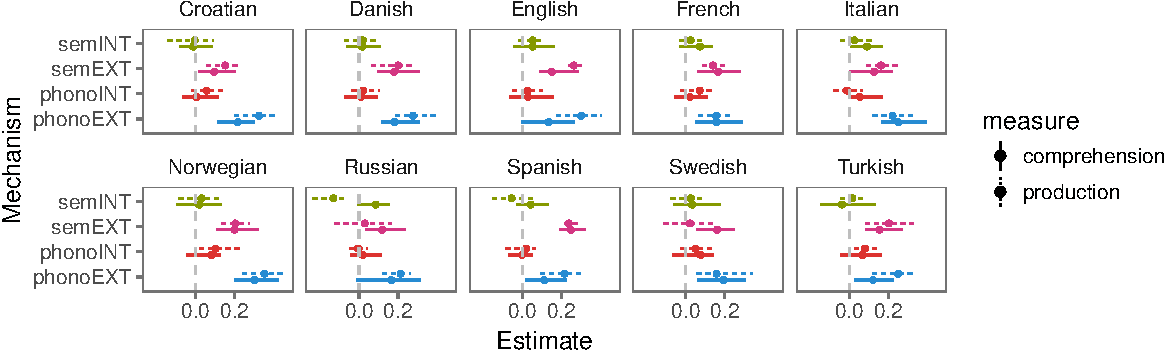
\includegraphics[width=\textwidth]{ms_files/figure-latex/growthPred-1} \caption{Evaluation of growth scenarios (EXT: externally-driven, INT: internally-driven) for both semantic and phonological networks. Each point represents the mean of the posterior distribution of the growth parameter, with ranges representing 95\% credible intervals. Positive values mean that learning proceeds according to the predictions of the growth scenario, whereas negative values mean that learning proceeds in opposition to the predictions of the growth scenario.}\label{fig:growthPred}
\end{figure}

\subsection{Network growth models}\label{network-growth-models}

To test the network growth scenarios, we fit two growth models to the
data. We calculated the probability that a word \(w_i\), with a utility
value \(u_i\) would enter the lexicon at a given month, using a softmax
function:

\begin{equation}
 p(w_i)= \frac{e^{\beta u_i}}{\sum_j e^{\beta u_j} }
\end{equation}

\noindent where \(\beta\) is a fitted parameter that captures the
magnitude of the relationship between network parameters and growth
(analogous to a regression coefficient). A positive value of \(\beta\)
means that words with higher utility values \(u_i\) are acquired first,
and a negative value means that words with lower utility values are
acquired first (see Figure \ref{fig:growth} for an illustration of how
utility values \(u_i\) are defined in each growth scenario). The
normalization includes all words that could be learned at that month.

We estimated the parameter \(\beta\) using a Bayesian approach. The
inference was performed using the probabilistic programming language
WebPPL (N. Goodman \& Stuhlmuller, 2014). We defined a uniform prior
over \(\beta\), and at each month, we computed the likelihood function
over words that could possibly enter the lexicon at that month, fit to
the words that have been learned at that month (using Formula 1). Markov
Chain Monte Carlo sampling resulted in a posterior distribution over
\(\beta\), which we summarized in Figure \ref{fig:growthPred}. The
results replicate Hills et al.'s original finding regarding the semantic
network in English and the production-based vocabulary, which is that
this network grows by EXT, not by INT. Crucially, our results show that,
generally speaking, this finding generalizes to comprehension-based
vocabulary, and holds across languages. This generalization was obtained
in both the semantic\footnote{One could imagine that the fact of using
  English free association norms cross-linguistically would decrease the
  effect of non-English semantic networks because of possible cultural
  differences. However, our findings do not support this assumption;
  rather, it supports our initial approximation about the shared nature
  of the semantic similarity measure. That said, this approximation is
  not perfect. For example, there is evidence that a small part of the
  variance in free association data can be explained by phonological
  similarity (Kachergis, Cox, \& Jones, 2011; Matusevych \& Stevenson,
  2018), thus leading to possibly minor cross-linguistic differences.}
and phonological domains.

\begin{figure}[!h]
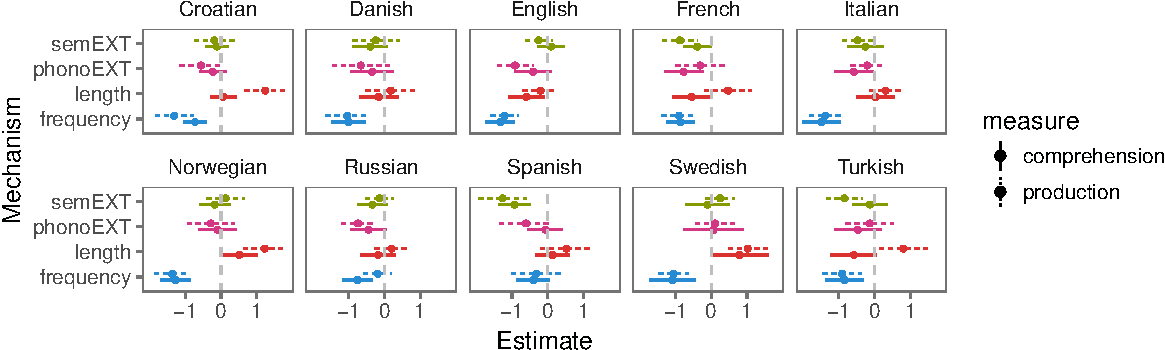
\includegraphics[width=\textwidth]{ms_files/figure-latex/staticPred-1} \caption{Estimates of the relative contribution of each predictor of AoA in the regression model in each language. Results are shown for both production and comprehension data. Ranges indicate 95\% confidence intervals. Positive values indicate a positive relationship (e.g. longer words tend to have a higher AoA), while negative values indicate a negative relationship (e.g. words with higher frequency tend to have a lower AoA).}\label{fig:staticPred}
\end{figure}

\begin{figure}[!h]
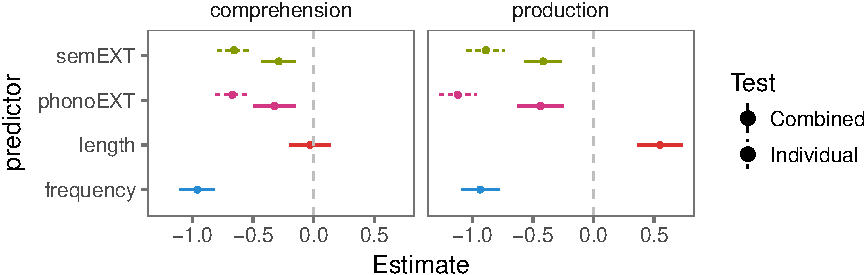
\includegraphics[width=\textwidth]{ms_files/figure-latex/staticAll-1} \caption{Estimates of the relative contribution of each predictor of AoA in the combined mixed-effects model with language as a random effect. Results are shown for both production and comprehension data. Ranges indicate 95\% confidence intervals. Dotted ranges indicate the estimates for the predictor in a separate model that includes only this predictor as a fixed effect.}\label{fig:staticAll}
\end{figure}

\subsection{Comparison to other predictors of age of
acquisition}\label{comparison-to-other-predictors-of-age-of-acquisition}

Above we showed that the way semantic and phonological information is
structured in the learning environment contributes to noun learning (via
EXT) across languages. However, we know that other factors influence
learning as well (e.g., Braginsky et al., 2019). Next, we investigated
how semantic and phonological connectivity interact with two other
factors. The first one is word frequency, a well-studied factor shown to
predict the age of acquisition in a reliable fashion (e.g., J. C.
Goodman et al., 2008). The second factor is word length, which was shown
to correlate with phonological connectivity: Shorter words are more
likely to have higher connectivity (Pisoni, Nusbaum, Luce, \&
Slowiaczek, 1985; Vitevitch \& Rodríguez, 2005).

Since we found INT to be uninformative, we dropped it from this
analysis, keeping only EXT. This simplified the model because we no
longer needed to fit growth month-by-month. The latter was a requirement
only for INT where the words' utilities varied from month to month,
depending on how connectivity changed in the growing internal network. A
more direct way to assess and compare the contribution of EXT in
relation to other word-level factors is through conducting regressions,
where connectivity in the learning environment, frequency, and length
predict the age of acquisition.

For word length, we counted the number of phonemes in our generated IPA
transcription. For word frequency, we used the frequency estimates from
Braginsky et al. (2019) where unigram counts were derived based on
CHILDES corpora in each language (MacWhinney, 2014). Although these
frequency counts use transcripts from independent sets of children, they
are based on large samples, and this allows us to average out possible
differences between children and the specificities of their input (see
J. C. Goodman et al., 2008 for a similar research strategy).

We conducted two analyses. We fit a linear regression for each language,
and we fit a linear mixed-effect model to all the data pooled across
languages, with language as a random effect. Figure \ref{fig:staticPred}
shows the coefficient estimate for each predictor in each language for
production and comprehension data. Figure \ref{fig:staticAll} shows the
coefficient estimates for all languages combined (all predictors were
centered and scaled).

The findings for the new predictors were as follows. Overall, frequency
is the largest and most consistent predictor of age of acquisition in
both comprehension and production data and across languages, endorsing
results for nouns across a variety of analyses (Braginsky et al., 2019;
J. C. Goodman et al., 2008; B. C. Roy et al., 2015). Word length is more
predictive for production than comprehension (and this difference is
very clear in the global model), replicating previous work (Braginsky et
al., 2019). Thus, word length seems to reflect the effects of
production's constraints rather than comprehension's constraints, i.e.,
longer words are harder to articulate but they may not be significantly
more difficult to store and access.

As for the factors of interest, i.e., semantic and phonological
connectivity, we found cross-linguistic differences. Connectivity
contributes to learning in some languages but not in other. In
particular, semantic connectivity does not explain variance in English
data beyond that explained by phonological connectivity, frequency and
length. This finding contrasts with the original finding in Hills et al.
(2009). However, this difference might be due to our using a slightly
different model (which included word length as a covariate) and a larger
dataset. That said, and despite these apparent cross-linguistic
differences, both phonological and semantic connectivity are significant
predictors in the combined model (Figure \ref{fig:staticAll}).

\section{Discussion}\label{discussion}

This study provided an analysis of network growth during development. We
compared two network growth scenarios described in the pioneering work
of Steyvers and Tenenbaum (2005) and Hills et al. (2009). The first
scenario, INT (originally called Preferential Attachment), described a
rich-get-richer network growth model in which the current structure of
the learner's internal network determines future growth; the other, EXT
(originally called Preferential Acquisition) described a model in which
the external, global environmental network structure determines
learners' growth patterns. These two mechanisms represent two
fundamentally different accounts of lexical growth: One suggests that
future word knowledge is primarily shaped by the children's past
knowledge and its organization, whereas the other suggests that learning
is shaped, rather, by salient properties in the input regardless of how
past knowledge is organized. The present study tested the generality of
previous findings by 1) investigating phonological networks together
with semantic networks, 2) testing both comprehension- and
production-based vocabularies, and 3) comparing the results across 10
languages.

We found that the original findings reported in Hills et al. (2009)
generalize well across all these dimensions. First, just like semantic
networks, phonological networks grow via the externally-driven scenario
(EXT), not by the internally-driven mechanism (INT). Second,
comprehension-based vocabularies grow in a way similar to
production-based vocabularies. Finally, the findings were, overall,
similar across the 10 languages we tested. Although we find some
cross-linguistic variation when semantic and phonological networks were
pitted against frequency and length, this variability is to be taken
with a grain of salt as it might be exaggerated in our study by several
factors such as the limited and partially-overlapping set of nouns for
each language, measurement error due to the sample of acquisition data,
the sample of frequency data, and the translation of association norms.
In fact, both phonological and semantic connectivity are significant
predictors above and beyond frequency and length when data are pooled
across languages.

These findings corroborate the hypothesis that children start by
learning words that have high similarity to a variety of other words in
the learning environment, not in the child's available lexicon. This
hypothesis implies that children are sensitive to highly connected words
although they do not initially have access to the full network, thus
raising some important questions: What mechanism allows children to
distinguish highly connected words from other words? Besides, why would
highly connected words be easier to learn?

One possibility is that these patterns emerge from children's use of
statistical learning abilities (Aslin \& Newport, 2012; Saffran, Aslin,
\& Newport, 1996; Smith \& Yu, 2008). The term \enquote{statistical
learning} has been used in the developmental literature to describes the
process by which one acquires information about their environment
through tracking the frequency distribution of some elements (e.g.,
words) in different contexts. An important property of this kind of
learning is that it occurs without explicit instructions and through
mere exposure to the input. Previous work in this line of research has
documented specific mechanisms which can explain the patterns found in
the current study.

For example, in the semantic domain, growth according to EXT could be
explained by a mechanism similar to cross-situational learning (McMurray
et al., 2012; Smith \& Yu, 2008; Yurovsky \& Frank, 2015). According to
this mechanism, children track the co-occurrence of concrete nouns with
their possible semantic referents. The referent of a word heard in only
one naming situation can be ambiguous (e.g., when the word
\enquote{ball} is heard for the first time in the presence of both a
ball and a chair), but hearing the same word in a diversity of semantic
contexts allows the learner to narrow down the set of possible
word-object mappings. In our case, free association (used to determine
semantic network connectivity) is related to contextual co-occurrence
(Fourtassi \& Dupoux, 2013; Griffiths, Steyvers, \& Tenenbaum, 2007),
meaning that highly connected words will tend to occur in a variety of
speech and referential contexts. This fact makes such words easier to
learn because they have more referential disambiguating cues across
learning contexts. Crucially, children can learn these words without
necessarily knowing the meaning of all other words with which they
co-occur (hence the similarity with EXT). This possibility is supported
by the finding that words' diversity of occurrence in child-directed
speech predicts their age of learning (Hills et al., 2010; Stella et
al., 2017).

In the phonological case, network growth according to EXT is also
compatible with a scenario whereby children are tracking low-level
statistical patterns, e.g., high probability sound sequences. Indeed,
connectivity in the phonological network is inherently correlated with
phonotactic probability (Vitevitch, Luce, Pisoni, \& Auer, 1999). That
is, highly connected words tend to be made of frequent sound sequences.
Children are sensitive to local phonotactic regularities (Jusczyk, Luce,
\& Charles-Luce, 1994), and this sensitivity might lead them to learn
higher-probability words more easily (Storkel, 2001). This explanation
is supported by computational simulations that show how learning general
phonotactics patterns create \enquote{well-worn paths} which allow the
models to represent several distinct but phonologically neighboring
words (Dell, Juliano, \& Govindjee, 1993; Siew, 2013; Takac, Knott, \&
Stokes, 2017). More generally, there is a growing interest in
investigating precisely how the local patterns acquired through
statistical learning may give rise to the global network organization
(For a review, see Karuza, Thompson-Schill, \& Bassett, 2016).

Besides using their own statistical learning skills, children could also
benefit from the way their caregivers speak. Perhaps the caregivers put
more emphasis on the words that are highly connected in \emph{their}
mature lexical network. This emphasis would guide children to learn
first these highly connected words, even though children do not have
access to the distribution of words' connectivity in the final network.
Investigating this possibility would require further research on
caregiver-child interaction (MacWhinney, 2014; B. C. Roy et al., 2015),
examining what words are introduced over development and the extent to
which children's uptake is influenced by this input (Clark, 2007; Hoff
\& Naigles, 2002; Huttenlocher et al., 1991).

This study investigated the class of nouns in isolation --- following
previous studies investigating the early semantic and phonological
network (Hills et al., 2009; Storkel, 2009). We could ask if studying
one class separately is a legitimate research strategy. In other words,
would word classes (such as nouns, verbs and function words) be acquired
relatively differently, or would they interact substantially to the
extent that it becomes unreasonable to study each class separately?

There are many observations that support the hypothesis that different
word classes have different pathways of learning, making it worthwhile
to study each class separately. For instance, different word classes
follow different time trajectories: In the early stages of development,
nouns tend to be acquired at a higher pace than predicates and function
words (Bates et al., 1994). Research has shown that this difference
cannot be trivially attributed to differences in the degree to which
these classes are present in the input; if anything, verbs and function
words are often more frequent in the input than nouns (e.g., Gentner,
1982). J. C. Goodman et al. (2008) found an effect of frequency on the
age of acquisition within --- not across --- classes. Further, recent
work by Braginsky et al. (2019) tested a large number of predictors,
besides frequency, and found that these predictors do not influence the
acquisition of word classes in the same way. For example, the
acquisition of nouns was found to be most influenced by frequency and
concreteness, whereas the acquisition of function words was most
influenced by word length.

This work shares a number of limitations with previous studies using
similar research strategy and datasets. Chief among these limitations is
the fact that the age of word acquisition is computed using different
children at different ages (due to the fact that available CDI data is
mainly cross-sectional). Such a measure has been shown to be valid and
reliable (Fenson et al., 1994), and has allowed researchers to study
important aspects of word learning (Braginsky et al., 2019; J. C.
Goodman et al., 2008; Hills et al., 2009; Stella et al., 2017; Storkel,
2009). In our case, the use of cost-effective cross-sectional data has
allowed us to leverage large-scale studies across several languages.
That said, it is important to remember that this type of data can only
inform us about the learning trajectory of the \enquote{average} child.
Although our study endorses, overall, the externally-driven account of
network growth, this does not mean individual children never use some
variant of INT or some combination of both INT and EXT (Beckage \&
Colunga, under review). To illustrate, some children develop
\enquote{islands of expertise,} that is, well-organized knowledge about
a certain topic (e.g., birds or dinosaurs). This prior knowledge enables
these children to learn new related words more easily (e.g., Chi \&
Koeske, 1983).

To conclude, our work validates and generalizes previous results in
early network development. It suggests that the advantage of highly
connected words may result, at least in the early stages of word
learning, from the operation of simpler mechanisms in both the semantic
and phonological domains. One question for future experimental work is
whether such correlational patterns of growth can be produced in
controlled behavioral experiments.

\vspace{1em}

\fbox{\parbox[b][][c]{14cm}{\centering All data and code for these analyses are available at\ \url{https://github.com/afourtassi/networks}}}
\vspace{1em}

\section{Acknowledgements}\label{acknowledgements}

This work was supported by a post-doctoral grant from the Fyssen
Foundation, NSF \#1528526, and NSF \#1659585.

\section{Disclosure statement}\label{disclosure-statement}

None of the authors have any financial interest or a conflict of
interest regarding this work and this submission.

\clearpage

\section{Appendix A: Analyses using different phnonological
distances}\label{appendix-a-analyses-using-different-phnonological-distances}

In the methods section, we based the choice of setting the threshold of
edit distance at 2 on the fact that the early lexicon is very sparse in
terms of phonological neighborhood; the early proposal that set the
threshold at 1 (e.g., Vitevitch, 2008) was defined in the context of
rather mature, dense lexicon. Increasing the threshold from 1 to 2
allows for a more reasonable representation of the similarity space of
the early phonological network.

That said, it is useful to include the results obtained with both
thresholds. In addition, it could be useful to compare the results to
the case of weighted networks, i.e., with no thresholding. The main
analyses for these two cases are shown in what follows. In summary, both
methods of constructing the phonological networks had issues. While the
fact of using an edit distance of 1 created sparsity, using weighted
networks created collinearity with length in the models.

\subsection{Analyses using phonological networks constructed with an
edit distance of
1}\label{analyses-using-phonological-networks-constructed-with-an-edit-distance-of-1}

We show in Figure \ref{fig:corrPlot} the correlation between the
phonological connectivity and age of acquisition in both comprehension
and production. The sparsity issue --- due to the low phonological
neighborhood in the children's lexicon --- is apparent: Most words had 0
connectivity, and a few had non-zero but small degrees. The values of
the correlations are much lower than the ones obtained with the
threshold of 2.

The next figures show how the phonology-based mechanism of growth
(phonoEXT) fares in comaprison to semEXT and other predictors of
learning in each language (Figure \ref{fig:staticPredEdit1} and across
all languages (Figure \ref{fig:staticAllEdit}). These figures show that
phonoEXT based on edit distance 1 had no noticeable effect on learning.

\begin{figure}[!h]
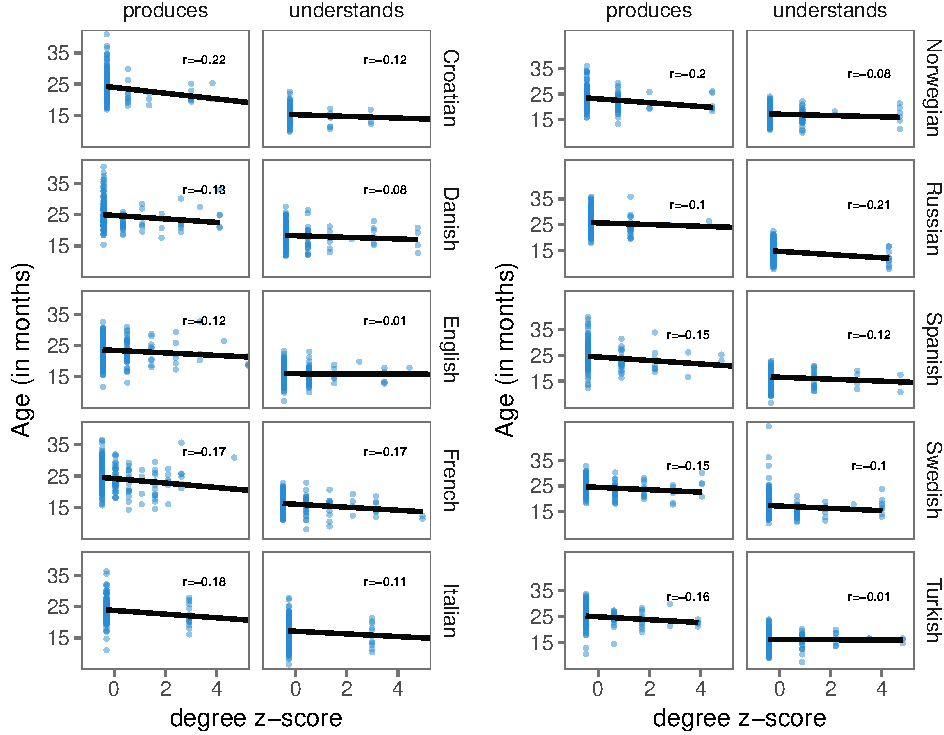
\includegraphics[width=\textwidth]{ms_files/figure-latex/corrPlot-1} \caption{Age of acquistion in both comprehension and production as predicted by the degree (i.e., connectivity) in the phonological networks, using an edit distance of 1. Each point is a word, with lines indicating linear model fits, and numbers indicating the Pearson correlation coefficients.}\label{fig:corrPlot}
\end{figure}

\begin{figure}[!h]
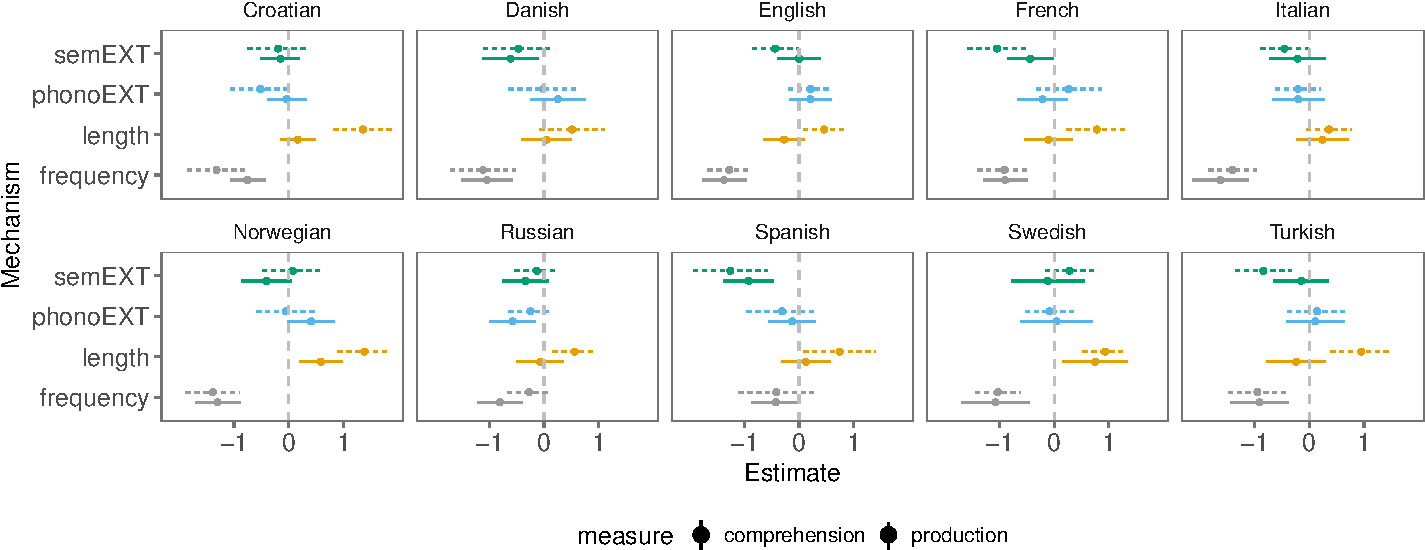
\includegraphics[width=\textwidth]{ms_files/figure-latex/staticPredEdit1-1} \caption{Estimates of the relative contribution of each predictor of AoA in the regression models. The phonologocal networks were based on an edit distance of 1. Ranges indicate 95\% confidence intervals. Positive values indicate a positive relationship (e.g. longer words tend to have a higher AoA), while negative values indicate a negative relationship (e.g. words with higher frequency tend to have a lower AoA).}\label{fig:staticPredEdit1}
\end{figure}

\begin{figure}[!h]
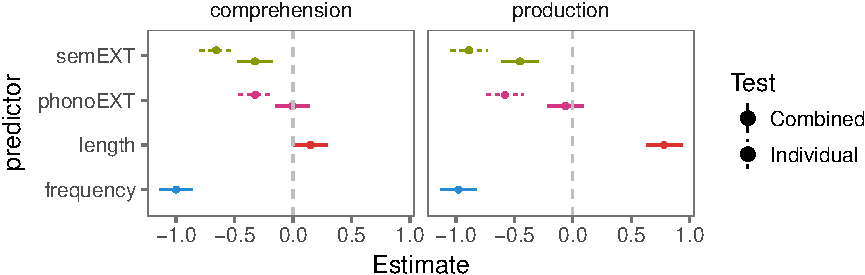
\includegraphics[width=\textwidth]{ms_files/figure-latex/staticAllEdit-1} \caption{Estimates of the relative contribution of each predictor of AoA in the combined model. The phonologocal networks were based on an edit distance of 1. Ranges indicate 95\% confidence intervals. Dotted ranges indicate the estimates for the predictor in a separate model that includes only this predictor as a fixed effect.}\label{fig:staticAllEdit}
\end{figure}

\subsection{Analyses using weighted phonological networks with no
thresholding}\label{analyses-using-weighted-phonological-networks-with-no-thresholding}

We constructed weighted phonological networks where the edge between a
given pair of words \((w_1, w_2)\) was wieghted by
\(\frac{1}{edit(w_1,w_2)}\). The phonological connectivity of a given
word \(w\) was defined as the sum over all weighted edges with every
other word \(w_i\) in the network, i.e.,
\(\sum_{i} \frac{1}{edit(w,w_i)}\).

The results were as follows. On the one hand, the correlations were
generally high and in many cases (especially in the production data),
higher than the ones obtained with the thresholds 2 and 1 (Figure
\ref{fig:corrPlotnt}). On the other hand, phonoEXT resulted in very
noisy estimates when we controlled for frequency and length (Figures
\ref{fig:staticPrednt} and \ref{fig:staticAllnt}). The reason was that
the new phonological connectivity was very highly correlated with
length. The average correlation across languages was \(r =\) -0.95 for
production data (compared to -0.29 and -0.60 for the phonological
networks with an edit distance of 1 and 2, respectvely). This fact lead
to a collinearity issue in the regression, making the effects hard to
estimate and interpret.

\begin{figure}[!h]
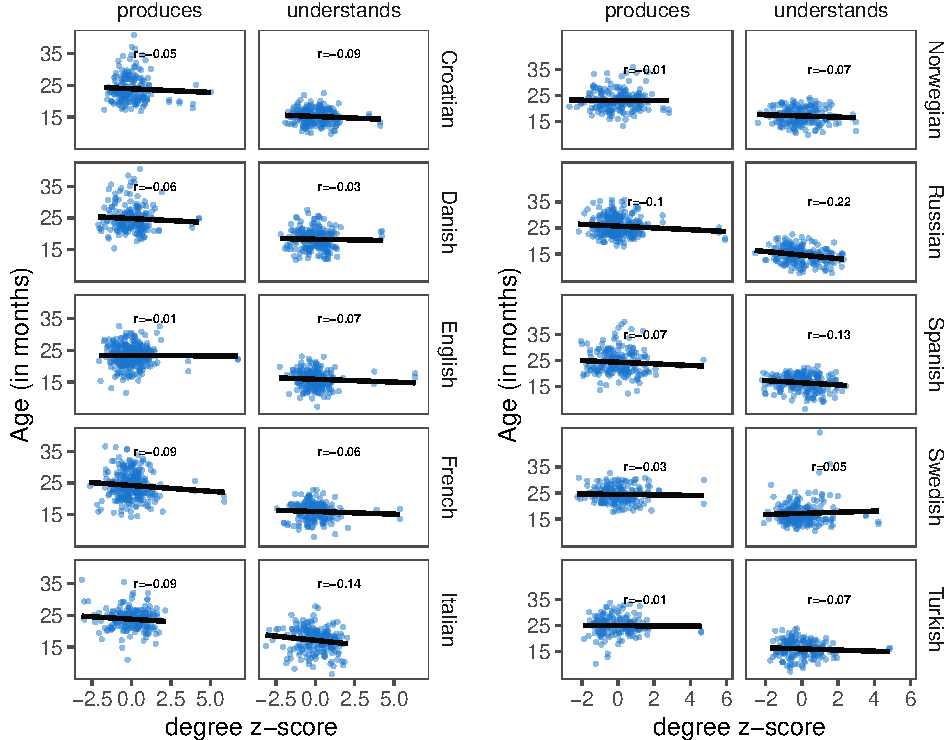
\includegraphics[width=\textwidth]{ms_files/figure-latex/corrPlotnt-1} \caption{Age of acquistion in both comprehension and production as predicted by the connectivity in the phonological network, using weighted edges. Each point is a word, with lines indicating linear model fits, and numbers indicating the Pearson correlation coefficients.}\label{fig:corrPlotnt}
\end{figure}

\begin{figure}[!h]
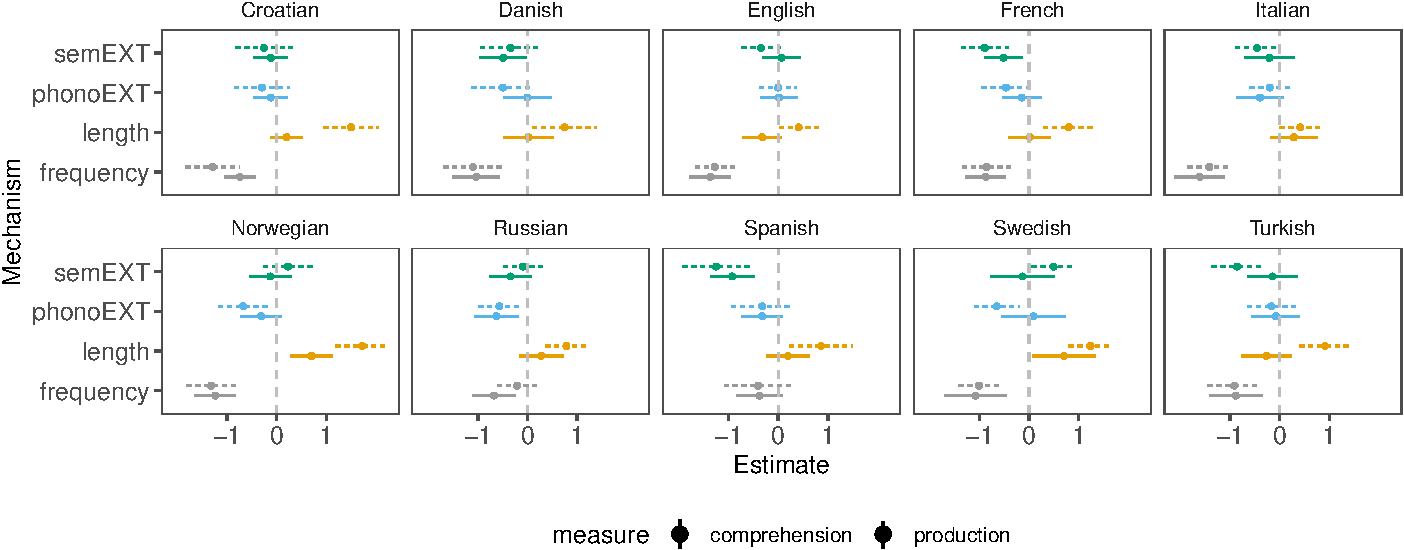
\includegraphics[width=\textwidth]{ms_files/figure-latex/staticPrednt-1} \caption{Estimates of the relative contribution of each predictor of AoA in the regression models. In the phonological networks, the edges between pairs of words were weighted by the inverse of the edit distance. Ranges indicate 95\% confidence intervals. Positive values indicate a positive relationship (e.g., longer words tend to have a higher AoA), while negative values indicate a negative relationship (e.g., words with higher frequency tend to have a lower AoA).}\label{fig:staticPrednt}
\end{figure}

\begin{figure}[!h]
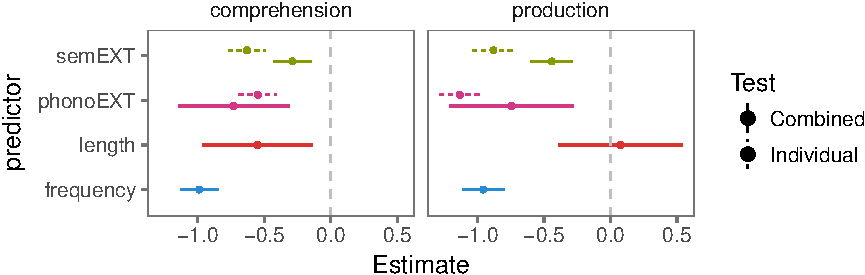
\includegraphics[width=\textwidth]{ms_files/figure-latex/staticAllnt-1} \caption{Estimates of the relative contribution of each predictor of AoA in the combined model. In the phonological networks, the edges between pairs of words were weighted by the inverse of the edit distance. Ranges indicate 95\% confidence intervals. Dotted ranges indicate the estimates for the predictor in a separate model that includes only this predictor as a fixed effect.}\label{fig:staticAllnt}
\end{figure}

\clearpage

\section{Appendix B: Phonological connectivity across
languages}\label{appendix-b-phonological-connectivity-across-languages}

We were interested in investigating if, for a given meaning (e.g.,
\enquote{dog} in English and \enquote{chien} in French), phonological
connectivity varied across languages. For example, if \enquote{dog} is
highly connected in the English phonological network, will
\enquote{chien} also be highly connected in the French network, or will
these two forms be situated independently in their relative phonological
networks?

If the phonological networks are very similar across languages, then
network growth in the phonological domain may be deeply intertwined with
growth in the semantic domain, rather than being an independent
mechanism of acquisition. If, instead, the phonological connectivity is
different from language to language, then this fact would lend support
to phonological growth being an independent driving mechanism of early
word learning.

To test this hypothesis, we compute the correlation of the unilemma's
phonological connectivity between every pair of languages. In Figure
\ref{fig:corrPair}, we plot the distribution of the pairwise Pearson
correlation coefficient. Generally speaking, languages are not highly
correlated at the phonological level as the distributions peak at low
values of \(r\), showing that phonological connectivity is not (at least
not fully) determined semantically.

\begin{figure}[!h]
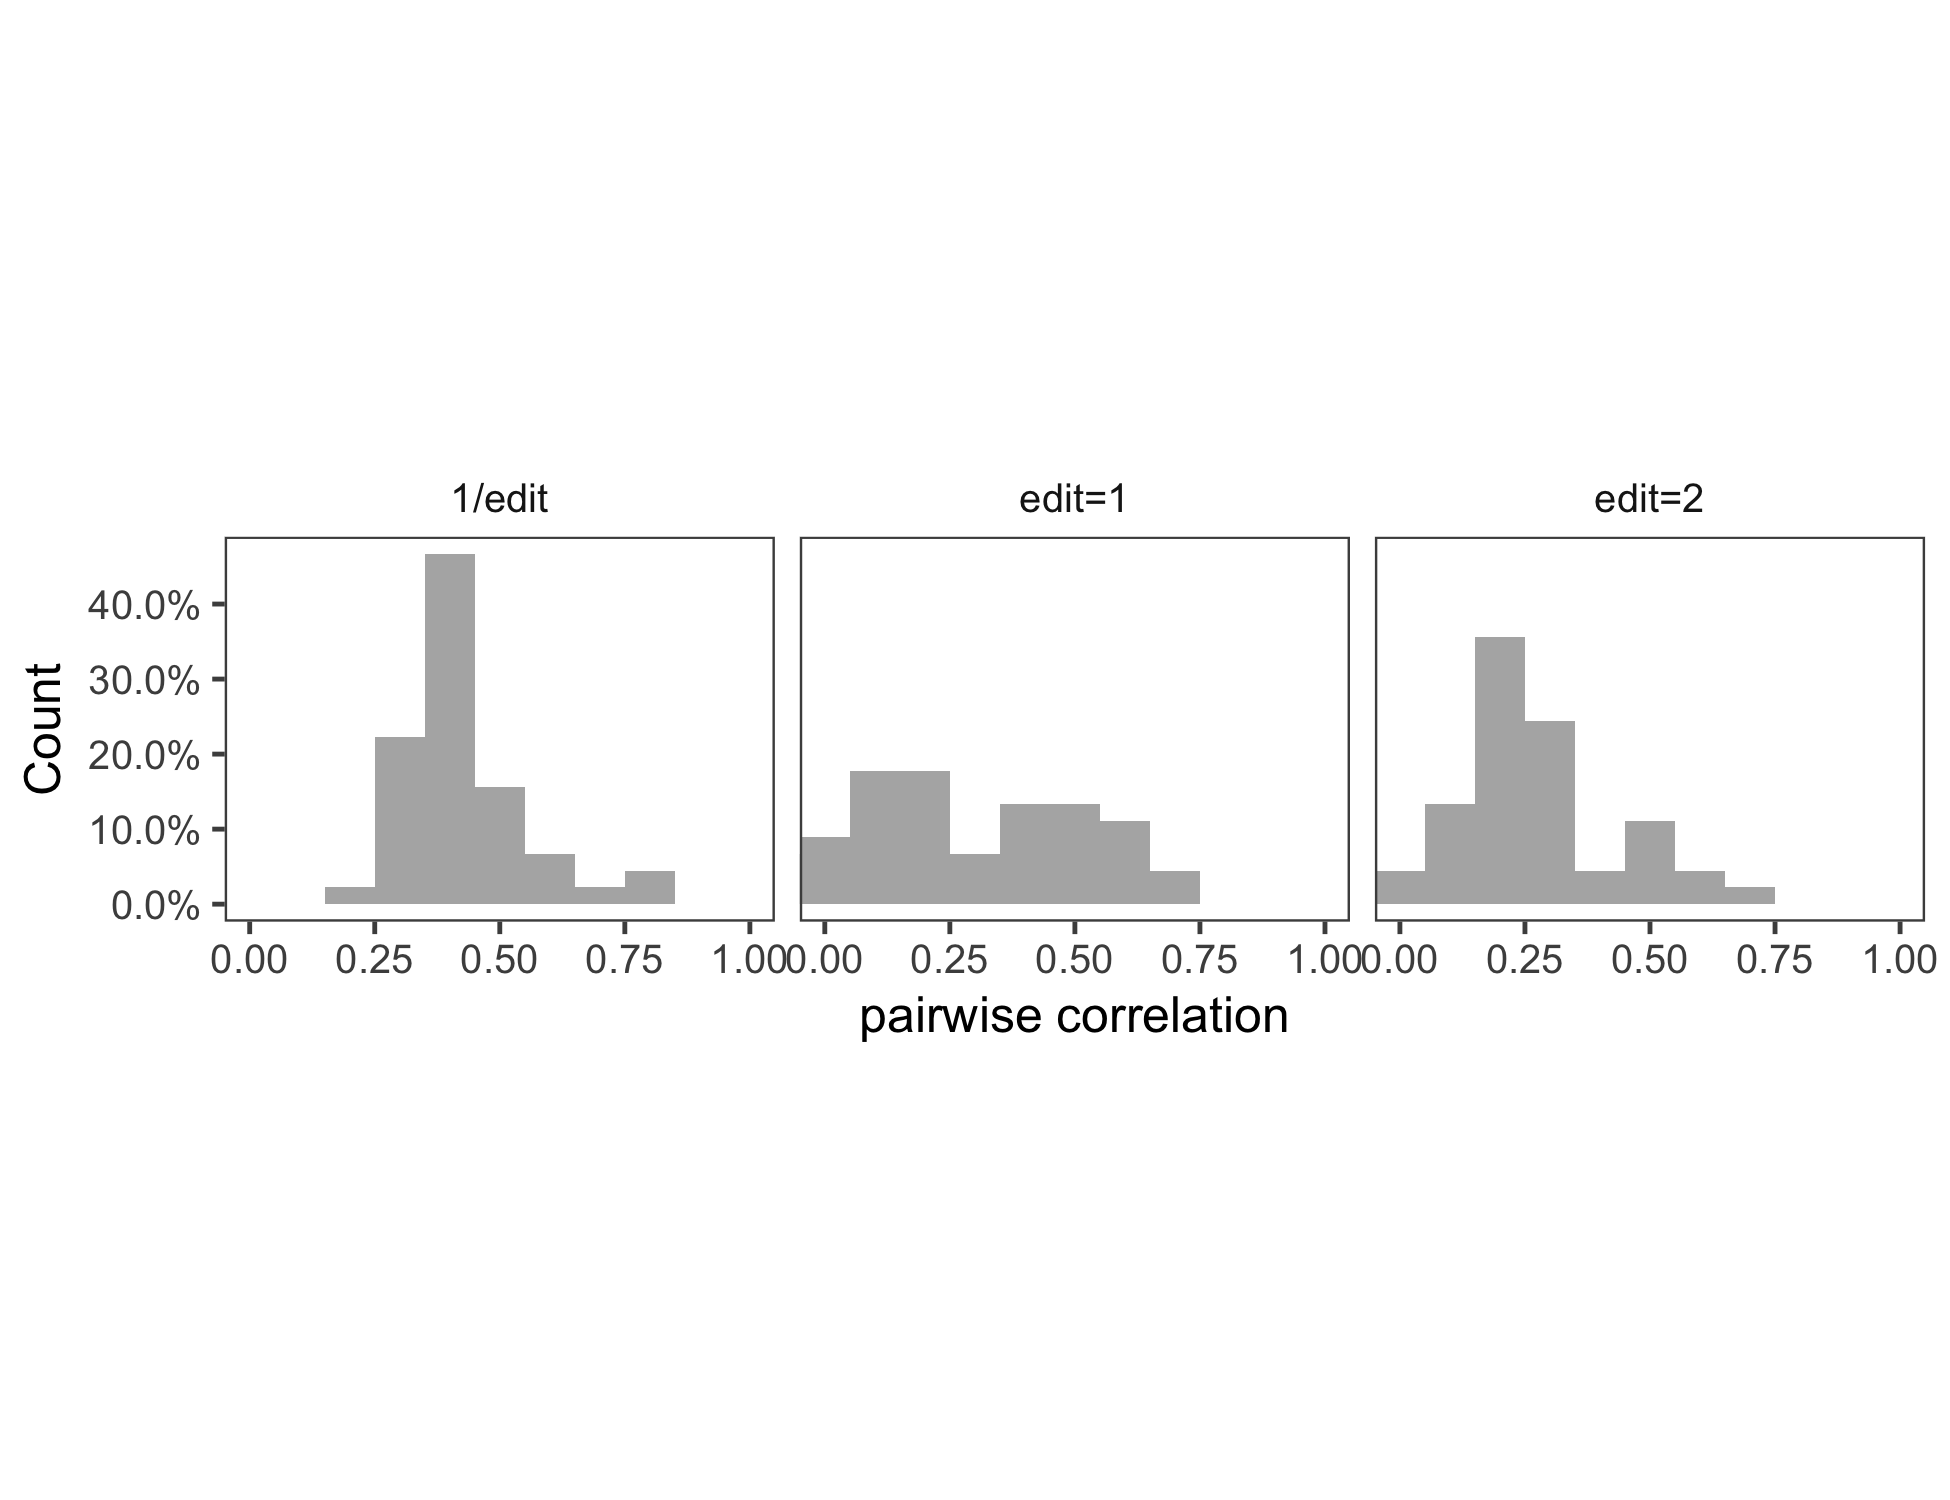
\includegraphics[width=\textwidth]{ms_files/figure-latex/corrPair-1} \caption{The distribution of the Pearson correlation coefficents of the unilemma's phonological connectivity between every pair of languages.}\label{fig:corrPair}
\end{figure}

\newpage 

\section{References}\label{references}

\setlength{\parindent}{-0.5in} \setlength{\leftskip}{0.5in}

\hypertarget{refs}{}
\hypertarget{ref-altvater2013}{}
Altvater-Mackensen, N., \& Mani, N. (2013). Word-form familiarity
bootstraps infant speech segmentation. \emph{Developmental Science},
\emph{16}(6).

\hypertarget{ref-arbesman2010}{}
Arbesman, S., Strogatz, S. H., \& Vitevitch, M. S. (2010). The structure
of phonological networks across multiple languages. \emph{International
Journal of Bifurcation and Chaos}, \emph{20}(03), 679--685.

\hypertarget{ref-aslin2012}{}
Aslin, R. N., \& Newport, E. L. (2012). Statistical learning: From
acquiring specific items to forming general rules. \emph{Current
Directions in Psychological Science}, \emph{21}(3).

\hypertarget{ref-barabasi99}{}
Barabasi, A.-L., \& Albert, R. (1999). Emergence of scaling in random
networks. \emph{Science}, \emph{286}(5439), 509--512.

\hypertarget{ref-bates1987}{}
Bates, E., \& MacWhinney, B. (1987). Competition, variation, and
language learning. In B. MacWhinney (Ed.), \emph{Mechanisms of language
acquisition}. Erlbaum.

\hypertarget{ref-bates1995}{}
Bates, E., Dale, P. S., \& Thal, D. (1995). Individual differences and
their implications for theories of language development. In P. Fletcher
\& B. MacWhinney (Eds.), \emph{The handbook of child language}. Oxford,
England: Blackwell.

\hypertarget{ref-bates1994}{}
Bates, E., Marchman, V., Thal, D., Fenson, L., Dale, P., Reznick, J. S.,
\ldots{} Hartung, J. (1994). Developmental and stylistic variation in
the composition of early vocabulary. \emph{Journal of Child Language},
\emph{21}(1).

\hypertarget{ref-beckage2016}{}
Beckage, N. M., \& Colunga, E. (2016). Language networks as models of
cognition: Understanding cognition through language. In \emph{Towards a
theoretical framework for analyzing complex linguistic networks} (pp.
3--28). Springer.

\hypertarget{ref-beckage}{}
Beckage, N. M., \& Colunga, E. (under review). Network growth modeling
to capture individual lexical learning.

\hypertarget{ref-benedict1979}{}
Benedict, H. (1979). Early lexical development: Comprehension and
production. \emph{Journal of Child Language}, \emph{6}(2), 183--200.

\hypertarget{ref-borovsky2016}{}
Borovsky, A., Ellis, E. M., Evans, J. L., \& Elman, J. L. (2016).
Lexical leverage: Category knowledge boosts real-time novel word
recognition in 2-year-olds. \emph{Developmental Science}, \emph{19}(6).

\hypertarget{ref-braginsky2019}{}
Braginsky, M., Yurovsky, D., Marchman, V. A., \& Frank, M. C. (2019).
Consistency and variability in children?s word learning across
languages. \emph{Open Mind}, \emph{3}.

\hypertarget{ref-carlson2014}{}
Carlson, M. T., Sonderegger, M., \& Bane, M. (2014). How children
explore the phonological network in child-directed speech: A survival
analysis of children's first word productions. \emph{Journal of Memory
and Language}, \emph{75}, 159--180.

\hypertarget{ref-chi1983}{}
Chi, M. T., \& Koeske, R. D. (1983). Network representation of a child's
dinosaur knowledge. \emph{Developmental Psychology}, \emph{19}(1).

\hypertarget{ref-clark2007}{}
Clark, E. V. (2007). Young children's uptake of new words in
conversation. \emph{Language in Society}, \emph{36}(2).

\hypertarget{ref-clauset09}{}
Clauset, A., Shalizi, C. R., \& Newman, M. E. J. (2009). Power-law
distributions in empirical data. \emph{SIAM Review}, \emph{51}(4),
661--703.

\hypertarget{ref-collins1975}{}
Collins, A. M., \& Loftus, E. F. (1975). A spreading-activation theory
of semantic processing. \emph{Psychological Review}, \emph{82}(6).

\hypertarget{ref-cristia2017}{}
Cristia, A., Dupoux, E., Gurven, M., \& Stieglitz, J. (2017).
Child-directed speech is infrequent in a forager-farmer population: A
time allocation study. \emph{Child Development}.

\hypertarget{ref-dell1993}{}
Dell, G. S., Juliano, C., \& Govindjee, A. (1993). Structure and content
in language production: A theory of frame constraints in phonological
speech errors. \emph{Cognitive Science}, \emph{17}(2), 149--195.

\hypertarget{ref-fenson94}{}
Fenson, L., Dale, P. S., Reznick, J. S., Bates, E., Thal, D. J.,
Pethick, S. J., \ldots{} Stiles, J. (1994). Variability in early
communicative development. \emph{Monographs of the Society for Research
in Child Development}, \emph{59}(5).

\hypertarget{ref-fourtassi2013}{}
Fourtassi, A., \& Dupoux, E. (2013). A corpus-based evaluation method
for distributional semantic models. In \emph{51st annual meeting of the
association for computational linguistics proceedings of the student
research workshop} (pp. 165--171).

\hypertarget{ref-frank2017}{}
Frank, M. C., Braginsky, M., Yurovsky, D., \& Marchman, V. A. (2017).
Wordbank: An open repository for developmental vocabulary data.
\emph{Journal of Child Language}, \emph{44}(3), 677--694.

\hypertarget{ref-gentner1982}{}
Gentner, D. (1982). Why nouns are learned before verbs: Linguistic
relativity versus natural partitioning. \emph{Center for the Study of
Reading Technical Report}.

\hypertarget{ref-gillespie15}{}
Gillespie, C. S. (2015). Fitting heavy tailed distributions: The
poweRlaw package. \emph{Journal of Statistical Software}, \emph{64}(2),
1--16. Retrieved from \url{http://www.jstatsoft.org/v64/i02/}

\hypertarget{ref-goodman2008}{}
Goodman, J. C., Dale, P. S., \& Li, P. (2008). Does frequency count?
Parental input and the acquisition of vocabulary. \emph{Journal of Child
Language}, \emph{35}(3), 515--531.

\hypertarget{ref-dippl}{}
Goodman, N., \& Stuhlmuller, A. (2014). The Design and Implementation of
Probabilistic Programming Languages. \url{http://dippl.org}.

\hypertarget{ref-griffiths07}{}
Griffiths, T. L., Steyvers, M., \& Tenenbaum, J. B. (2007). Topics in
semantic representation. \emph{Psychological Review}, \emph{114}(2),
2007.

\hypertarget{ref-hills2018}{}
Hills, T. T., \& Siew, C. S. (2018). Filling gaps in early word
learning. \emph{Nature Human Behaviour}, \emph{2}(9).

\hypertarget{ref-hills2010}{}
Hills, T. T., Maouene, J., Riordan, B., \& Smith, L. B. (2010). The
associative structure of language: Contextual diversity in early word
learning. \emph{Journal of Memory and Language}, \emph{63}(3), 259--273.

\hypertarget{ref-hills2009}{}
Hills, T. T., Maouene, M., Maouene, J., Sheya, A., \& Smith, L. (2009).
Longitudinal analysis of early semantic networks: Preferential
attachment or preferential acquisition? \emph{Psychological Science},
\emph{20}(6), 729--739.

\hypertarget{ref-hoff2002}{}
Hoff, E., \& Naigles, L. (2002). How children use input to acquire a
lexicon. \emph{Child Development}, \emph{73}(2).

\hypertarget{ref-huttenlocher1991}{}
Huttenlocher, J., Haight, W., Bryk, A., Seltzer, M., \& Lyons, T.
(1991). Early vocabulary growth: Relation to language input and gender.
\emph{Developmental Psychology}, \emph{27}(2).

\hypertarget{ref-jusczyk1994}{}
Jusczyk, P. W., Luce, P. A., \& Charles-Luce, J. (1994). Infant's
sensitivity to phonotactic patterns in the native language.
\emph{Journal of Memory and Language}, \emph{33}(5), 630--645.

\hypertarget{ref-kachergis2011}{}
Kachergis, G., Cox, G. E., \& Jones, M. N. (2011). OrBEAGLE: Integrating
orthography into a holographic model of the lexicon. In
\emph{International conference on artificial neural networks} (pp.
307--314). Springer.

\hypertarget{ref-karuza2016}{}
Karuza, E. A., Thompson-Schill, S. L., \& Bassett, D. S. (2016). Local
patterns to global architectures: Influences of network topology on
human learning. \emph{Trends in Cognitive Sciences}, \emph{20}(8).

\hypertarget{ref-kuhl1997}{}
Kuhl, P. K., Andruski, J. E., Chistovich, I. A., Chistovich, L. A.,
Kozhevnikova, E. V., Ryskina, V. L., \ldots{} Lacerda, F. (1997).
Cross-language analysis of phonetic units in language addressed to
infants. \emph{Science}, \emph{277}(5326), 684--686.

\hypertarget{ref-luce1998}{}
Luce, P. A., \& Pisoni, D. B. (1998). Recognizing spoken words: The
neighborhood activation model. \emph{Ear and Hearing}, \emph{19}(1).

\hypertarget{ref-lupyan2017}{}
Lupyan, G., \& Lewis, M. (2017). From words-as-mappings to
words-as-cues: The role of language in semantic knowledge.
\emph{Language, Cognition and Neuroscience}.

\hypertarget{ref-macwhinney2014}{}
MacWhinney, B. (2014). \emph{The CHILDES project: Tools for analyzing
talk, Volume II}. Psychology Press.

\hypertarget{ref-markman90}{}
Markman, E. M. (1990). Constraints children place on word meanings.
\emph{Cognitive Science}, \emph{14}(1), 57--77.

\hypertarget{ref-matusevych2018}{}
Matusevych, Y., \& Stevenson, S. (2018). Analyzing and modeling free
word associations. In \emph{Proceedings of the 40th Annual Conference of
the Cognitive Science Society}.

\hypertarget{ref-mcmurray2012}{}
McMurray, B., Horst, J. S., \& Samuelson, L. K. (2012). Word learning
emerges from the interaction of online referent selection and slow
associative learning. \emph{Psychological Review}, \emph{119}.

\hypertarget{ref-mcrae2005}{}
McRae, K., Cree, G. S., Seidenberg, M. S., \& McNorgan, C. (2005).
Semantic feature production norms for a large set of living and
nonliving things. \emph{Behavior Research Methods}, \emph{37}(4),
547--559.

\hypertarget{ref-nelson1998}{}
Nelson, D. L., McEvoy, C. L., \& Schreiber, T. A. (1998). \emph{The
University of South Florida word association, rhyme, and word fragment
norms}. Retrieved from \url{http://w3.usf.edu/FreeAssociation/}

\hypertarget{ref-pisoni1985}{}
Pisoni, D. B., Nusbaum, H. C., Luce, P. A., \& Slowiaczek, L. M. (1985).
Speech perception, word recognition and the structure of the lexicon.
\emph{Speech Communication}, \emph{4}(1), 75--95.

\hypertarget{ref-roy2015}{}
Roy, B. C., Frank, M. C., DeCamp, P., Miller, M., \& Roy, D. (2015).
Predicting the birth of a spoken word. \emph{Proceedings of the National
Academy of Sciences}, \emph{112}(41).

\hypertarget{ref-saffran1996}{}
Saffran, J. R., Aslin, R. N., \& Newport, E. L. (1996). Statistical
learning by 8-month-old infants. \emph{Science}, \emph{274}(5294),
1926--1928.

\hypertarget{ref-siew2013}{}
Siew, C. S. (2013). Community structure in the phonological network.
\emph{Frontiers in Psychology}, \emph{4}.

\hypertarget{ref-slobin2014}{}
Slobin, D. I. (2014). \emph{The crosslinguistic study of language
acquisition} (Vol. 4). Psychology Press.

\hypertarget{ref-smith2008}{}
Smith, L., \& Yu, C. (2008). Infants rapidly learn word-referent
mappings via cross-situational statistics. \emph{Cognition},
\emph{106}(3).

\hypertarget{ref-stella2017}{}
Stella, M., Beckage, N. M., \& Brede, M. (2017). Multiplex lexical
networks reveal patterns in early word acquisition in children.
\emph{Scientific Reports}, \emph{7}.

\hypertarget{ref-steyvers2005}{}
Steyvers, M., \& Tenenbaum, J. B. (2005). The large-scale structure of
semantic networks: Statistical analyses and a model of semantic growth.
\emph{Cognitive Science}, \emph{29}(1), 41--78.

\hypertarget{ref-storkel2001}{}
Storkel, H. L. (2001). Learning new words: Phonotactic probability in
language development. \emph{Journal of Speech, Language, and Hearing
Research}, \emph{44}(6), 1321--1337.

\hypertarget{ref-storkel2009}{}
Storkel, H. L. (2009). Developmental differences in the effects of
phonological, lexical and semantic variables on word learning by
infants. \emph{Journal of Child Language}, \emph{36}(2), 29--321.

\hypertarget{ref-swingley2018}{}
Swingley, D., \& Humphrey, C. (2018). Quantitative linguistic predictors
of infants' learning of specific english words. \emph{Child
Development}, \emph{89}(4).

\hypertarget{ref-takac2017}{}
Takac, M., Knott, A., \& Stokes, S. (2017). What can neighbourhood
density effects tell us about word learning? Insights from a
connectionist model of vocabulary development. \emph{Journal of Child
Language}, \emph{44}(2).

\hypertarget{ref-vitevitch2008}{}
Vitevitch, M. S. (2008). What can graph theory tell us about word
learning and lexical retrieval? \emph{Journal of Speech, Language, and
Hearing Research}, \emph{51}(2), 408--422.

\hypertarget{ref-vitevitch2005}{}
Vitevitch, M. S., \& Rodríguez, E. (2005). Neighborhood density effects
in spoken word recognition in spanish. \emph{Journal of Multilingual
Communication Disorders}, \emph{3}(1).

\hypertarget{ref-vitevitch1999}{}
Vitevitch, M. S., Luce, P. A., Pisoni, D. B., \& Auer, E. T. (1999).
Phonotactics, neighborhood activation, and lexical access for spoken
words. \emph{Brain and Language}, \emph{68}(1), 306--311.

\hypertarget{ref-youn2016}{}
Youn, H., Sutton, L., Smith, E., Moore, C., Wilkins, J. F., Maddieson,
I., \ldots{} Bhattacharya, T. (2016). On the universal structure of
human lexical semantics. \emph{Proceedings of the National Academy of
Sciences}, \emph{113}(7), 1766--1771.

\hypertarget{ref-yurovsky2015}{}
Yurovsky, D., \& Frank, M. C. (2015). An integrative account of
constraints on cross-situational learning. \emph{Cognition}, \emph{145}.






\end{document}
